% DOCX paragraph 626
\chapter[Agujeros negros]{Agujeros negros: los campeones de la curvatura}\label{ch:06}

% DOCX paragraph 627

% DOCX paragraph 630
En el capítulo anterior vimos que la aparición de la astronomía de rayos X\index{rayos X!radiación} a finales de la década de 1960 dejó «desconcertados» a los astrofísicos. Las observaciones obtenidas con satélites de rayos X\index{rayos X!radiación} revelaron la existencia de objetos nunca antes vistos, con masas muy grandes pero tamaños minúsculos. Fuentes como Sco X-1\index{Scorpius X-1 (Sco X-1)} y Cyg X-1\index{Cyg X-1} representaban sorpresas inexplicables para la astrofísica y ponían en cuestión todo lo que se sabía de la física moderna en aquel momento. Para colmo, para Sco X-1\index{Scorpius X-1 (Sco X-1)} se podía postular una explicación plausible recurriendo a una hipotética «estrella de neutrones», pero la fenomenología de Cyg X-1 planteaba un enigma mucho más desconcertante.

% DOCX paragraph 631
Con una masa de unas 15 masas solares, desde luego no se podía invocar la presencia de una estrella de neutrones para explicar las observaciones de Cyg X-1\index{Cyg X-1}. Además, la variabilidad\index{variabilidad} de la emisión de rayos X de Cyg X-1 (normalmente en torno a un segundo, aunque podía bajar hasta unos pocos milisegundos) sugería la presencia de un objeto mucho más compacto, con un tamaño del orden de solo unas pocas decenas de kilómetros. Hoy sabemos que Cyg X-1 es un representante bastante corriente de toda una clase de objetos celestes que presentan la misma fenomenología: las binarias de rayos X de alta masa (HMXB). De nuevo, se trata de sistemas binarios en los que hay una transferencia de masa desde una estrella normal hacia otro objeto muchísimo más compacto. Igual que ocurre con Sco X-1\index{Scorpius X-1 (Sco X-1)}, la transferencia de materia en el caso de Cyg X-1 tiene lugar a través de un disco de acreción\index{disco de acreción} por el que la materia cae sobre el objeto compacto, se calienta y emite una radiación\index{rayos X!radiación}\index{rayos X!radiación}\index{rayos X!radiación} muy intensa en la banda de rayos X. La diferencia más relevante entre Cyg X-1 y Sco X-1\index{Scorpius X-1 (Sco X-1)} es que, en el caso de Cyg X-1, la estrella normal era el objeto de mayor masa, mientras que el otro miembro de la binaria, más compacto, es lo que hoy conocemos como… ¡un agujero negro!

% DOCX paragraph 632
Estos cuerpos celestes se han convertido en parte integrante de la imaginación colectiva y la cultura general. Hasta tal punto que mi pequeña hija Anna, que entonces aún no tenía edad de ir al colegio, dio una respuesta astuta (y divertida) a la sencilla pregunta: «¿Qué es un agujero negro?». Como suelen hacer los niños, abordó la pregunta con la superioridad típica de quien piensa que lo sabe todo de la vida: «Bueno, ¡es obvio! Es simplemente un agujero que no se puede llenar…». Esta respuesta no es errónea; en realidad, es absolutamente cierta, porque normalmente un agujero se puede llenar. Sin embargo, no deja de ser una descripción puramente cualitativa que, por desgracia, no explica qué son los agujeros negros. Dado que no es raro que la información que encontramos sobre ellos sea confusa o incluso engañosa, puede ser conveniente poner un poco de orden en lo que quizá ya sabes.

% DOCX paragraph 633
Así pues, para eliminar algunos mitos urbanos y las descripciones más superficiales de los agujeros negros, me propongo ofrecer una explicación clara y cada vez más detallada de lo que son y de las propiedades que poseen. Comenzaré con su génesis y terminaré hablando de las dificultades a las que todavía se enfrentan los científicos al manejar un concepto que, en el fondo, resulta difícil de aceptar.

% DOCX paragraph 638
\section{Una solución del todo extravagante}\label{sec:06-solution}

% DOCX paragraph 640
Un planteamiento sencillo pero riguroso para explicar los agujeros negros podría partir de su definición y, en particular, de la fascinante, aunque trágica, génesis de lo que resultó ser la primera solución de las ecuaciones de Einstein, hallada por Karl\index{Schwarzschild!Karl} Schwarzschild (1873-1916), un físico de Fráncfort del Meno.

% DOCX paragraph 641
Recordemos que en noviembre de 1915, en las actas de la entonces Real Academia de Ciencias de Berlín, Albert Einstein publicó sus ecuaciones de campo, el fundamento de su teoría de la relatividad general\index{relatividad general}. En aquella época, Karl Schwarzschild ya era un astrónomo célebre: era el director del Observatorio Astrofísico de Potsdam, a unos pocos kilómetros de Berlín. A pesar de ocupar un cargo tan prestigioso, Schwarzschild, como muchos judíos alemanes de su generación, sentía la necesidad de expresar su lealtad a Alemania y el sentido de pertenencia que lo vinculaba a la sociedad alemana. Por eso, cuando estalló la Primera Guerra Mundial en 1914, se alistó como voluntario y fue enviado a combatir. Aunque ya tenía 40 años, lo destinaron al frente occidental y después al oriental. Por desgracia, debido a las duras condiciones que encontró en Rusia, enfermó gravemente y su salud se deterioró con rapidez. Falleció en 1916, pero en los últimos meses de su vida consiguió encontrar la primera solución de las ecuaciones de Einstein.

% DOCX paragraph 642
Sin ser consciente de la repercusión que iba a tener, Schwarzschild no puso nombre a su solución\index{Schwarzschild!solución}. En 1967 (otro suceso significativo de aquel año…), el físico estadounidense John Archibald Wheeler utilizó el término descriptivo «agujero negro\index{Schwarzschild!agujero negro}».\textsuperscript{\hyperlink{note:06-01}{1}} Aunque los hallazgos de Schwarzschild representan la solución más sencilla de las ecuaciones de campo de la relatividad general, en el curso que imparto sobre esta teoría en Fráncfort solo puedo abordar el tema en la parte final, tras haber dedicado meses a introducir todas las matemáticas necesarias para derivarla. Déjame recordarte las tres hipótesis importantes bajo las cuales se puede obtener esta solución:

% DOCX paragraph 644
\begin{enumerate}
\item la presencia de una simetría esférica\index{simetría esférica};

% DOCX paragraph 645
\item la independencia del tiempo, es decir, la solución es estática;

% DOCX paragraph 646
\item la ausencia de materia, es decir, la solución es en el vacío\index{vacío}.
\end{enumerate}

% DOCX paragraph 648
Ahora sabemos que la de Schwarzschild es también la única solución de las ecuaciones de Einstein que satisface estas condiciones (esta es la tesis del famoso teorema de George Birkhoff\index{Birkhoff, George}, del que hablaremos más adelante). Sin embargo, es poco probable que el propio Schwarzschild apreciara plenamente la novedad radical o las implicaciones de su solución. Como muchos científicos después de él, debió de considerarla una «rareza» de la nueva teoría, hasta el punto de iniciar enseguida una intensa correspondencia con Einstein para pedirle su opinión.

% DOCX paragraph 649
Hay varios aspectos de la solución de Schwarzschild que hacen que parezca, cuando menos, bastante extraña. En primer lugar, tiene simetría esférica y, por tanto, posee un «centro» y una región «lejana» (llamada también región asintótica). En esta región, es decir, a grandes distancias del centro, la solución de Schwarzschild no es especialmente extraña, pues es la misma que la de una fuente de gravedad en la teoría de la gravedad de Newton. Ahora bien, mientras que en la teoría de Newton este resultado solo es posible en presencia de materia (porque un objeto con masa tiene que producir el campo gravitatorio), la solución de Schwarzschild es, como se ha dicho, en el vacío\index{vacío}. En esencia, sugiere que es posible crear un campo gravitatorio a partir de… ¡nada! Una idea decididamente extravagante.\index{espaciotiempo!asintótico}

% DOCX paragraph 650
Una segunda rareza es que predice la existencia de una superficie esférica con radio \emph{r=r\textsubscript{S}}, cuyo valor viene dado por la siguiente ecuación:

% DOCX paragraph 652
\begin{equation}\label{eq:06-01}
r_{S}=2M\textcolor{gray}{\frac{G}{c^{2}}}
\end{equation}

% DOCX paragraph 654
Precisamente en este radio\index{Schwarzschild!radio}, llamado también radio de Schwarzschild y que representa una de las escalas de longitud fundamentales en astronomía, ocurren una serie de fenómenos extraños de los que hablaremos enseguida. Sin embargo, el más peculiar e inquietante es que la solución de Schwarzschild no está bien definida en ese radio. Desde un punto de vista matemático, las funciones que describen la solución en él divergen, es decir, toman valores infinitamente grandes.

% DOCX paragraph 655
Se ve a primera vista que la ecuación \eqref{eq:06-01} nos dice que el radio de Schwarzschild es igual al doble de la masa \emph{M} del objeto en cuestión, es decir, el agujero negro (de nuevo, he puesto en gris las constantes que no tienen un «significado físico»). Hoy sabemos que el radio de Schwarzschild \emph{r\textsubscript{S}} representa el radio del llamado \emph{horizonte de sucesos\index{horizonte de sucesos}} (volveremos sobre esto) y que la divergencia de la solución en ese radio no es especialmente preocupante: es simplemente el resultado de una elección inadecuada de coordenadas\index{coordenadas}\index{singularidad!de coordenadas}. De hecho, se puede utilizar todo un conjunto de coordenadas más apropiadas que «eliminan» esta singularidad y hacen que el radio \emph{r=2GM/c\textsuperscript{2}} sea perfectamente regular, es decir, sin divergencias.

% DOCX paragraph 656
Sin embargo, en el radio de Schwarzschild quedan otras peculiaridades. En particular, es imposible que un rayo de luz emitido en ese radio (y también cualquier objeto con masa) se desplace hacia fuera, a radios mayores, aunque el rayo sí puede desplazarse hacia dentro. En otras palabras, la superficie esférica cuyo radio es igual al de Schwarzschild se comporta como una membrana unidireccional: permite absorber objetos, pero no deja escapar nada. Más adelante veremos qué significa esto desde el punto de vista físico.

% DOCX paragraph 657
Por último, una tercera rareza de la solución de Schwarzschild ---la que entraña las complicaciones más graves--- es que también diverge en el centro, es decir, en \emph{r=0}. Sin embargo, a diferencia de la singularidad en el horizonte, la del centro es mucho más grave y no se puede «curar», ni siquiera mediante una transformación inteligente de las coordenadas\index{coordenadas}. Por el contrario, todos los indicadores posibles de lo que ocurre al acercarse al radio cero sugieren que allí todas las magnitudes físicas y geométricas se vuelven infinitamente grandes. Por eso, \emph{r=0} recibe el nombre fascinante, aunque algo inquietante, de \emph{singularidad del espaciotiempo}.

% DOCX paragraph 658
Hoy llamamos \emph{singularidad física\index{singularidad!física}} al punto \emph{r=0} de la solución de Schwarzschild: un punto del espaciotiempo donde las ecuaciones de la relatividad general\index{relatividad general} son imposibles de resolver porque divergen. Esto significa, a su vez, que cerca de la singularidad las leyes de la física\index{singularidad!física} dejan de ser válidas y, por tanto, no podemos predecir ni siquiera comprender lo que podría ocurrir allí. La singularidad física sigue siendo la mayor piedra en el zapato de la teoría de Einstein: la manifestación inequívoca de que, por correcta que sea, sigue siendo incompleta. En efecto, aunque se ha demostrado que la relatividad general proporciona predicciones correctas sobre el comportamiento de la gravedad a gran escala, sigue sin poder describirla en presencia de dimensiones muy pequeñas y grandes curvaturas, es decir, en escalas en las que entran en juego las leyes de la mecánica cuántica\index{mecánica cuántica}. Aún hoy, pese a los esfuerzos de generaciones de físicos teóricos, carecemos de una teoría de la gravedad cuántica\index{gravedad cuántica}. Pero no te inquietes: volveremos a este punto al final de nuestro viaje.

% DOCX paragraph 659
Así pues, cuando se propuso en 1916, la solución de Schwarzschild provocó reacciones encontradas. Por una parte, mostraba que las ecuaciones de Einstein eran extremadamente interesantes y tenían soluciones; por otra, planteaba más preguntas que respuestas. Como puedes imaginar, dadas sus rarezas, quizá la solución de Schwarzschild fue una mala manera de empezar a comprender las consecuencias de la relatividad general\index{relatividad general}. Tal vez por eso la comunidad científica de aquellos años recibió la nueva teoría propuesta por Einstein con una actitud de interés distante y curiosidad escéptica. Esto valía tanto para los matemáticos, atraídos por las implicaciones geométricas de la teoría, como para los físicos, interesados, en cambio, en sus repercusiones experimentales.

% DOCX paragraph 660
El clima científico de aquellos años se caracterizaba por una cortés apreciación de la teoría, junto con una indiferencia de fondo hacia ella, agravada por la dificultad de encontrar soluciones y, por tanto, de comprender sus predicciones. Así, la teoría de la relatividad general se convirtió en «víctima» de una falta generalizada de interés por parte de la comunidad científica. Sin embargo, esta actitud no era irracional y estaba alimentada, en parte, por algunas «distracciones» importantes. En aquella época, una teoría igualmente atractiva había comenzado a llamar la atención de los físicos: la mecánica cuántica\index{mecánica cuántica}, otra teoría fascinante que pretendía desvelar las propiedades de las partículas elementales. También era extraña, pero tenía la gran ventaja de ofrecer predicciones mucho más fáciles de entender y, sobre todo, de verificar mediante experimentos.

% DOCX paragraph 661
Como resultado, durante los primeros años de su existencia, la teoría de Einstein parecía condenada a caer lentamente en el olvido. Por fortuna, la llegada de la astronomía de rayos X\index{rayos X!radiación} y la observación de objetos como Cyg X-1\index{Cyg X-1} obligaron a la comunidad científica, cincuenta años después, a reconsiderar sus predicciones.

% DOCX paragraph 664
\section[Velocidad de escape y horizonte de sucesos]{Velocidad de escape, horizonte de sucesos y singularidades}\label{sec:06-escape}

% DOCX paragraph 666
Tras repasar las principales rarezas de la solución de Schwarzschild, intentaremos ahora comprenderlas. En particular, hablaremos del horizonte de sucesos, de las peculiares propiedades de esta superficie matemática y, por último, de la singularidad física\index{singularidad!física} en el centro de un agujero negro.

% DOCX paragraph 667
En primer lugar, para ilustrar las características del horizonte de sucesos\index{horizonte de sucesos}, conviene partir de un fenómeno que podemos experimentar directamente. Imaginemos que tomamos una pelota de tenis y la golpeamos hacia arriba, procurando que su trayectoria sea lo más vertical posible. Observaremos que, dada una cierta velocidad inicial, la pelota se frena. Más precisamente, su velocidad disminuye de forma progresiva durante el ascenso hasta hacerse cero en un punto concreto de su movimiento vertical. En ese momento, la pelota deja de subir y cae, acelerando a medida que vuelve hacia ti. Sabemos que la altura máxima que alcanza está directamente relacionada con la fuerza con la que la hemos golpeado. En efecto, si volvemos a lanzarla con otra velocidad, cambiará la altura máxima que alcanza antes de invertir su movimiento. En particular, esa altura será menor si la velocidad inicial es menor, y mayor si la velocidad de partida es mayor. Está claro, por tanto, que hay una relación precisa entre la velocidad inicial con la que golpeamos la pelota y la altura máxima a la que llega. En física nos gusta pensar que esa altura representa la posición en la que la energía cinética inicial de la pelota (la energía que tiene por su movimiento) se convierte por completo en energía potencial gravitatoria, es decir, la energía que tiene por su posición.

% DOCX paragraph 668
El aspecto más importante de este sencillo ejemplo es que hay una razón por la que la pelota de tenis vuelve a caer: está \emph{ligada\index{gravitatoriamente!ligada} gravitatoriamente\index{gravitatoriamente!no ligada}}. Dicho de otro modo, el campo gravitatorio producido por la Tierra domina tanto la dinámica de la pelota que esta no puede escapar de él. Siguiendo este razonamiento, cabe preguntarse si podríamos darle una velocidad inicial que le permitiera escapar del campo gravitatorio o dejar de estar ligada a él. La respuesta es sí, y es lo que llamamos, sin demasiada sorpresa, \emph{velocidad de escape\index{velocidad de escape}}. Calcular su valor es bastante sencillo y requiere comparar la energía cinética\index{energia@energía!cinética} con la energía potencial\index{energia@energía!potencial (gravitatoria)} gravitatoria. De esta forma obtenemos una expresión válida tanto en la teoría de la gravedad de Newton como en la de Einstein, a saber:

% DOCX paragraph 670
\begin{equation}\label{eq:06-02}
v_{f}=\sqrt{2\frac{M}{R}\textcolor{gray}{G}}
\end{equation}

% DOCX paragraph 672
La expresión anterior nos dice que, dada una fuente de campo gravitatorio con masa \emph{M} y radio \emph{R} (por ejemplo, la Tierra), la velocidad de escape es proporcional a la raíz cuadrada de la masa e inversamente proporcional a la raíz cuadrada del radio de la fuente. La velocidad de escape aumenta con la masa del planeta (cuanto más masivo sea, mayor será la velocidad necesaria para escapar de él) y disminuye a medida que aumenta su tamaño.

% DOCX paragraph 673
Veámoslo con unos números. Si quisiéramos golpear nuestra pelota de tenis de manera que escapara del campo gravitatorio terrestre, tendríamos que lanzarla a una velocidad de 11,2 kilómetros por segundo, o 40\,320 kilómetros por hora. Una velocidad tan alta que ni el mejor tenista podría jamás poner una pelota en órbita en nuestro planeta. Lo cual es una suerte, porque ¡sería muy frustrante ver un partido de tenis en el que los jugadores no pudieran golpear la pelota demasiado alto por miedo a perderla!

% DOCX paragraph 674
Dicho esto, la ecuación \eqref{eq:06-02} es interesante al menos por dos razones. La primera es que la velocidad de escape\index{velocidad de escape} es independiente de la masa de la pelota que golpeamos (en la fórmula solo aparece la masa de la fuente del campo gravitatorio). En otras palabras, para enviar a la Luna\index{Luna} un grano de arena o una nave espacial se necesita la misma velocidad (obviamente, la energía empleada sería muy distinta…). La segunda razón es que, como quizá hayas advertido, la velocidad de escape depende de una magnitud con la que ya nos hemos encontrado: la compacidad \emph{M/R} de la fuente del campo gravitatorio. Esto significa que los distintos objetos celestes (la Tierra, la Luna, el Sol…) tendrán diferentes velocidades de escape porque sus compacidades y, por tanto, sus campos gravitatorios son distintos. En efecto, la velocidad de escape en la Luna es casi cinco veces menor que en la Tierra: unos 2,4 kilómetros por segundo. Por tanto, ni siquiera en nuestro satélite natural podríamos golpear la pelota para sacarla del campo gravitatorio con la mera fuerza de nuestros músculos, pero sin duda conseguiríamos lanzarla mucho más alto que en la Tierra. En cambio, si intentáramos hacerlo en el Sol, ya resultaría difícil lanzarla hacia arriba, pues allí la velocidad de escape es de unos 615 kilómetros por segundo.

% DOCX paragraph 675
Por cierto, el hecho de que la velocidad de escape en la Luna\index{Luna} sea tan baja ---menor que la velocidad media de las moléculas de nitrógeno gaseoso--- explica por qué la Luna no tiene atmósfera. Por suerte para nosotros, la velocidad de escape de la Tierra es suficientemente alta para haber retenido una atmósfera, cuya presencia es esencial para la vida en nuestro planeta.

% DOCX paragraph 678
\section[La máxima velocidad de escape]{Cuando la velocidad de escape es la máxima posible}\label{sec:06-light}

% DOCX paragraph 680
Hay otro aspecto de la ecuación \eqref{eq:06-02} que merece destacarse. Sabemos que existe una velocidad máxima\index{compacidad!máxima (absoluta)} a la que se pueden mover los objetos: la velocidad de la luz. Así pues, podemos utilizar la fórmula \eqref{eq:06-02} para calcular la compacidad \emph{M/R} para la cual la velocidad de escape\index{velocidad de escape} es igual a la de la luz. Si lo hacemos, descubriremos que, ignorando las constantes \emph{G} y \emph{c}\textsuperscript{2}, el valor de la compacidad es \emph{M/R=1/2}. Este resultado hace mucho más fácil entender el radio de Schwarzschild, dado por la ecuación \eqref{eq:06-01}: es el radio de un objeto, más concretamente un agujero negro\index{compacidad!agujero negro}, cuya compacidad es \emph{M/R=1/2}, la mayor que hemos visto hasta ahora. Esto nos permite introducir una nueva definición del horizonte de sucesos\index{horizonte de sucesos} como la superficie en la que la velocidad de escape es la máxima posible, es decir, la de la luz. En otras palabras, si se emitiera exactamente desde el horizonte de sucesos, la luz no podría abandonar el campo gravitatorio del agujero negro, porque necesitaría una velocidad de escape superior a la máxima que permite la física.

% DOCX paragraph 681
Imagina ahora que estás sobre esta superficie matemática y emites un haz láser hacia una estrella lejana. Debido a la enorme intensidad del campo gravitatorio, el haz no puede propagarse hacia fuera y, en cambio, ¡tendrá que regresar! Debo insistir en que este comportamiento solo se daría si estuviéramos situados exactamente en el horizonte de sucesos. Si nos colocáramos un poco más afuera y repitiéramos el experimento, el campo gravitatorio seguiría siendo enormemente intenso, pero parte de nuestro haz láser conseguiría escapar y llegar a un observador situado a gran distancia.\textsuperscript{\hyperlink{note:06-02}{2}} Dicho de otro modo, este peculiar comportamiento de la luz solo se aplica mientras estamos en \emph{r=r\textsubscript{S}}; fuera del horizonte de sucesos, es decir, a radios mayores que \emph{r\textsubscript{S}}, el campo gravitatorio sigue siendo extremadamente intenso, pero no es «invencible». En cambio, si emitiéramos un haz de luz dentro del horizonte de sucesos, es decir, a radios menores que \emph{r\textsubscript{S}}, el haz solo se movería hacia dentro, en dirección al centro del agujero negro, donde se encuentra la singularidad física\index{singularidad!física}.

% DOCX paragraph 682
Pero volvamos al haz de luz emitido justo fuera del horizonte de sucesos. Hemos visto que parte de ese haz llegaría a un observador incluso a una distancia considerable, por ejemplo, en la Tierra. Sin embargo, la luz que percibiera ese observador sería muy diferente, en términos de color (o longitud de onda), de la emitida inicialmente. Supongamos que, al emitirse, la luz tenía una longitud de onda visible, digamos en la parte azul del espectro\index{espectro!electromagnético}. El observador situado a gran distancia, en cambio, ¡la recibiría en la parte roja del espectro visible!

% DOCX paragraph 683
Además, esta tendencia de la luz a «parecer roja» sería más fuerte cuanto más cerca del horizonte de sucesos se produjera la emisión. La longitud de onda de un haz de luz nos informa sobre la energía\index{energia@energía!fotón (del)}\index{foton@fotón!energía} de los fotones que lo componen; más precisamente, la energía de un fotón es inversamente proporcional a su longitud de onda. Este proceso de enrojecimiento revela que el haz pierde energía al propagarse desde su punto de emisión, cerca del horizonte de sucesos, hasta el observador lejano.

% DOCX paragraph 684
Este proceso, que parece tan extraño, cobra pleno sentido si volvemos a pensar en nuestra pelota de tenis golpeada hacia arriba. También la pelota, al ascender, pierde energía cinética, que se transforma en energía potencial gravitatoria. En un punto determinado se ve obligada a detenerse, al agotar toda su energía cinética, y tiene que volver a caer. Como un fotón\index{foton@fotón} no puede disminuir su velocidad, porque, por definición, está obligado a moverse a la velocidad de la luz, manifiesta esta pérdida de energía modificando su longitud de onda. Acabo de describir un fenómeno bien conocido en astrofísica, que refleja una propiedad muy común de la emisión de los objetos celestes compactos: el \emph{desplazamiento gravitatorio al rojo\index{desplazamiento al rojo (gravitatorio)}\index{gravitatorio!desplazamiento al rojo (véase desplazamiento al rojo)}}. Este fenómeno alcanza su extremo precisamente en los agujeros negros y se vuelve matemáticamente infinito para un fotón emitido desde el horizonte de sucesos. Si el desplazamiento al rojo de un fotón emitido en \emph{r=r\textsubscript{S}} es infinito, el observador nunca lo recibirá. Por tanto, el desplazamiento al rojo infinito que experimenta un fotón emitido en el horizonte de sucesos es otra manera de entender por qué no puede propagarse hacia fuera, sino, como mucho, permanecer en órbita\index{orbita@órbita}s tangentes a esa superficie.

% DOCX paragraph 685
Para que este concepto resulte lo más intuitivo posible, hagamos juntos un experimento mental. Imagina que estás a cierta distancia del horizonte de sucesos ---quizá a bordo de una nave espacial situada en una de las órbita\index{orbita@órbita!circular estable}s circulares estables que permiten las leyes de la relatividad general alrededor de un agujero negro--- y dejas caer hacia el cuerpo celeste un dispositivo parecido a la luz de una boya marina, que emite destellos a intervalos regulares. Pues bien, a medida que la boya se aleja de ti y se acerca al horizonte de sucesos, verás que el intervalo entre destellos aumenta, mientras que la luz que produce, inicialmente de un blanco intenso, se vuelve cada vez más roja. El proceso continuará mientras pueda llegarte un número suficiente de fotones, pero, con el paso del tiempo, recibirás cada vez menos y estarán cada vez más desplazados al rojo. En un momento dado, cuando la boya esté muy cerca del horizonte de sucesos, dejarás de ver luz alguna, por sensibles que sean tus instrumentos. ¡Pero eso no significa que el dispositivo haya dejado de funcionar o haya sido destruido antes de cruzar el horizonte! Si hubieras estado sujeto a la boya, habrías visto que sus destellos tenían siempre la misma periodicidad y que la luz no cambiaba de color en absoluto. Además, tras un intervalo de tiempo preciso y bastante sencillo de calcular, cruzarías el horizonte de sucesos y te encontrarías dentro de él, sin poder comunicarte con el universo exterior. Dependiendo de la masa del agujero negro, y especialmente si fuera supermasivo\index{agujero negro!supermasivo}, el paso por el horizonte ni siquiera iría acompañado de ningún acontecimiento particularmente dramático.\textsuperscript{\hyperlink{note:06-02}{2}}

% DOCX paragraph 686
Esta diferencia en la percepción\index{percepción}\index{observacional!percepción} de los procesos físicos por distintos observadores (es decir, tú observando la boya desde la nave y tú cayendo junto con la boya) es una propiedad auténtica de la relatividad general\index{relatividad general}, de la que deriva su nombre. Aunque esta «relatividad» de la percepción pueda parecer inquietante, desaparece cuando hablamos de los propios procesos físicos y no de cómo los percibimos al observarlos. En ese caso, todos los observadores estarán de acuerdo en la misma conclusión.

% DOCX paragraph 687
El ejemplo de la boya nos enseña que es imposible observar directamente un horizonte de sucesos (o el nacimiento de un agujero negro) mientras esas observaciones involucren fotones y, por tanto, la emisión y recepción de luz. Sin embargo, sigue siendo posible obtener pruebas indirectas de la presencia de un agujero negro, ya sea mediante la emisión de radiación electromagnética de sus proximidades (como veremos en el capítulo 7) o incluso sin luz alguna, mediante la emisión de ondas gravitatorias (como aprenderemos en el capítulo 8).

% DOCX paragraph 688
A estas alturas soy consciente de que te he dado mucha información sobre los agujeros negros y sus horizontes de sucesos. Déjame recapitular brevemente para poner un poco de orden y centrarnos en los puntos más esenciales de lo que hemos visto:\index{horizonte de sucesos}

% DOCX paragraph 690
\begin{itemize}
\item Se puede emitir un haz de luz hacia fuera desde un punto muy alejado y exterior al horizonte de sucesos: se propagará hasta regiones situadas a mayores distancias sin cambiar perceptiblemente su longitud de onda.

% DOCX paragraph 691
\item Se puede emitir un haz de luz hacia fuera desde un punto cercano al horizonte de sucesos, pero todavía exterior a él, aunque una parte se curvará hacia atrás y caerá sobre el horizonte. Cuanto más cerca de este se produzca la emisión, mayor será la cantidad de luz que no consiga propagarse hacia fuera.

% DOCX paragraph 692
\item La luz emitida cerca del horizonte de sucesos cambiará de longitud de onda y se volverá roja debido al desplazamiento gravitatorio al rojo\index{desplazamiento al rojo (gravitatorio)}. La intensidad de este desplazamiento aumenta cuando la emisión se produce desde puntos más próximos al horizonte y se vuelve infinita para un fotón emitido exactamente en esa superficie.

% DOCX paragraph 693
\item Un haz de luz emitido desde el horizonte de sucesos, es decir, desde un radio \emph{r=2M}, no puede propagarse hacia fuera: si el agujero negro no lo absorbe, su destino es permanecer para siempre tangente a esa superficie esférica.

% DOCX paragraph 694
\item A diferencia de la superficie de una estrella de neutrones, el horizonte de sucesos no es una superficie sólida, sino puramente matemática. Es la frontera que marca la transición entre dos procesos físicos: uno en el que un fotón\index{foton@fotón} consigue propagarse hacia fuera y otro en el que se ve obligado a «regresar».

% DOCX paragraph 695
\item Gran parte de lo dicho sobre los fotones también vale para los objetos con masa, que, al acercarse al horizonte de sucesos, necesitarán energías cada vez mayores para escapar del campo gravitatorio. La energía requerida se vuelve infinita si la partícula se encuentra exactamente sobre el horizonte de sucesos.
\end{itemize}

% DOCX paragraph 696
Concluiré esta discusión con una nota histórica. Ya he mencionado que la expresión de la velocidad de escape\index{velocidad de escape} \eqref{eq:06-02} es también la misma en la teoría de la gravedad de Newton y se conocía desde principios del siglo XVIII. De hecho, el naturalista británico John Michell\index{Michell, John} (1724-1793) fue el primero en formular lo que podría considerarse una idea temprana de un horizonte de sucesos. En un artículo publicado en 1783,\textsuperscript{\hyperlink{note:06-03}{3}} introdujo el concepto de «estrellas oscuras»: cuerpos celestes cuya compacidad era tal que la velocidad de escape igualaba a la de la luz. ¡Según esta extraordinaria anticipación, esas estrellas no serían capaces de emitir luz! Por supuesto, en 1783 aún estaba por llegar la relatividad general, así como el concepto de horizonte de sucesos, y las observaciones todavía no habían revelado la presencia de objetos como Cyg X-1\index{Cyg X-1}. Aun así, resulta increíble que se formularan ideas relacionadas con los agujeros negros, aunque de forma algo embrionaria, siglos antes de que estos conceptos adquirieran una definición precisa.

% DOCX paragraph 700
\section{Cuando el tiempo se burla de nosotros}\label{sec:06-time}

% DOCX paragraph 702
Ha llegado el momento de enfrentarnos a otro fenómeno físico que se da cerca del horizonte de sucesos y aparece una y otra vez en las películas de ciencia ficción con agujeros negros: la dilatación del tiempo\index{dilatación del tiempo}.\index{dilatación (del tiempo)|see{dilatación del tiempo}}

% DOCX paragraph 703
En el capítulo 4 vimos que, si la masa o la energía pueden curvar el espacio, es perfectamente plausible que ocurra lo mismo con el tiempo. Además, hemos dicho que la gravedad estira la longitud de onda de un fotón emitido cerca de un horizonte de sucesos\index{horizonte de sucesos} y dirigido hacia fuera, provocando lo que se conoce como desplazamiento gravitatorio al rojo\index{desplazamiento al rojo (gravitatorio)}. Ahora solo nos queda unir estos dos conceptos.

% DOCX paragraph 704
Para ello utilizaré dos observadoras hipotéticas, Anna y Emilia, cada una a bordo de su propia nave espacial, en órbita circular estable\index{orbita@órbita!circular estable} alrededor de un agujero negro, de manera que ninguna corre el riesgo de caer en él. Mantendrán una distancia constante al agujero negro, con Anna más cerca del horizonte de sucesos y Emilia más lejos. Supongamos ahora que Anna emite un haz de luz azul hacia Emilia: como hemos visto, esta última lo recibirá sin ningún problema, pero con una longitud de onda rojiza. Hemos interpretado el fenómeno como consecuencia de la energía que gasta el fotón al salir del pozo gravitatorio desde el que fue emitido. Sin embargo, hay otra forma de describirlo. Un fotón es una onda electromagnética, y el número de crestas asociadas a esa onda tiene que ser el mismo para Anna, que lo envió, y para Emilia, que lo recibió. Además, puesto que el fotón debe moverse a la velocidad de la luz, el cambio de longitud de onda puede interpretarse como una variación en el transcurso del tiempo medido por Anna y Emilia. En resumen, el hecho de que las dos observadoras registren frecuencia\index{foton@fotón!frecuencia}s distintas para el mismo fotón (recuerda que su frecuencia \emph{f} es inversamente proporcional a su longitud de onda \emph{λ}: \emph{f =c/λ}) puede interpretarse como consecuencia de que el tiempo empleado en contar el mismo número de crestas es distinto para cada observadora.

% DOCX paragraph 705
Ya nos encontramos con algo parecido en el capítulo 4, al hablar de la ligera diferencia entre los relojes situados en tierra y los colocados en satélites. Pues bien, como en aquel fenómeno, el desplazamiento gravitatorio al rojo\index{desplazamiento al rojo (gravitatorio)} que experimentan Anna y Emilia puede describirse como una manifestación de la elasticidad del tiempo. Si comparamos lo que ocurre con el GPS, la diferencia importante es que, al estar cerca de un agujero negro, donde la curvatura es extrema, Anna y Emilia registrarán una variación mucho mayor (posiblemente extrema) en el transcurso del tiempo. De hecho, esta diferencia divergirá cerca del horizonte de sucesos. Dicho de otro modo, el desplazamiento al rojo casi infinito de un fotón\index{foton@fotón} emitido cerca del horizonte puede interpretarse como resultado de la enorme «ralentización» del tiempo cuando el fotón intenta moverse hacia fuera. Para aclararlo: el observador situado a una distancia muy grande del agujero negro verá que el tiempo avanza al mismo ritmo que en un espaciotiempo plano. En cambio, para un observador cercano al agujero negro, el tiempo transcurre más despacio, porque esa región del espaciotiempo está mucho más curvada. En última instancia, el tiempo prácticamente se congelaría para un observador sobre el horizonte de sucesos.

% DOCX paragraph 706
Quizá necesitemos recurrir a otro experimento mental para comprender mejor el concepto. Esta vez, sin embargo, tendremos que estirar un poco más la imaginación, pues utilizaremos condiciones físicas extremas, aunque perfectamente plausibles.

% DOCX paragraph 707
Imaginemos, pues, a dos astronautas, Carolin y Dominik, a bordo de una nave espacial en órbita\index{orbita@órbita!circular estable} circular, a una distancia segura de un agujero negro supermasivo, por ejemplo, el que se encuentra en el centro de la galaxia\index{M87!galaxia} elíptica M87 (hablaré con más detalle de este fantástico objeto en el capítulo 7). Los dos astronautas están aburridos y deciden hacer una «excursión espacial» en la pequeña nave de servicio. Como gran parte de la acción de esa zona ocurre alrededor del agujero negro (de una u otra forma, ¡parece que todo acaba cayendo literalmente en él!), deciden acercarse, manteniéndose a una distancia segura del horizonte de sucesos. Ambos saben muy bien que existen órbitas seguras para la pequeña nave y que pueden calcularlas a partir de la potencia de sus motores. Tras comprobar que todo está en orden, escriben una nota en el diario electrónico de a bordo, anotan las coordenadas\index{coordenadas} exactas, incluida la fecha y la hora astrales, y abandonan la nave nodriza.

% DOCX paragraph 708
Los campos gravitatorios cerca de un agujero negro supermasivo\index{agujero negro!supermasivo}, como M87*\index{M87*}, varían de forma muy gradual. Más precisamente, el radio de curvatura cerca de estos objetos es extremadamente grande y las diferencias entre lugares próximos (es decir, los campos de marea) son bastante pequeñas. Por eso, en lugar de encender los cohetes de su nave, Carolin y Dominik deciden disfrutar simplemente de su «caída libre\index{caída libre}» mientras son atraídos hacia el centro de M87. Es como si descendieran poco a poco por una montaña de enormes dimensiones horizontales y pendiente muy suave. Sin embargo, la atracción gravitatoria del agujero negro es tan grande que, incluso sin motores, Carolin y Dominik alcanzan enseguida velocidades muy altas, próximas a la de la luz.

% DOCX paragraph 709
Mientras tanto, sorbiendo té caliente y saboreando unos pastelitos recién hechos, los dos astronautas disfrutan al contemplar por las ventanillas de la nave el impresionante panorama de la materia que converge con ellos hacia el agujero negro. Finalmente, deciden que es hora de volver, y los instrumentos confirman que, a esa distancia del horizonte de sucesos, aún pueden invertir el rumbo. Encienden los motores y orientan la nave hacia la nodriza, empleando, hay que decirlo, una cantidad considerable de energía para ascender por el pozo gravitatorio al que habían descendido poco a poco. En esencia, la parte difícil es la subida para alejarse del agujero negro…

% DOCX paragraph 710
Una vez en la nave nodriza, comprueban los instrumentos. El calendario indica una fecha astral muy distinta de aquella en la que partieron y de la que marca su pequeña nave: según el ordenador de la nodriza, la excursión ha durado varios meses. Carolin y Dominik, sin embargo, no se sorprenden; sabían que ocurriría, y por eso se llevaron los pastelitos recién hechos en lugar de dejarlos en el frigorífico de la nave. Por supuesto, allí el tiempo pasó mucho más deprisa que a bordo de la nave de servicio, pero para los dos astronautas era un fenómeno perfectamente normal y totalmente predecible. De hecho, antes de partir, Dominik había calculado el tiempo que «medirían» a bordo de la nave pequeña para llegar al horizonte de sucesos o, si decidieran cruzarlo, a la singularidad física\index{singularidad!física} del centro. Consciente de la diferencia entre «su» tiempo en la pequeña nave y el medido por los instrumentos de la nodriza, calculó la ruta procurando que la diferencia no fuera excesiva: no quería dejar la nave nodriza sin tripulación demasiado tiempo. En resumen, esta excursión revela que Carolin y Dominik conocen la relatividad general y las sutilezas del tiempo en campos gravitatorios intensos.

% DOCX paragraph 711
Que el tiempo pueda ir más despacio e incluso detenerse nos parece absurdo; por eso puede ser útil reflexionar sobre dos aspectos importantes del fenómeno. En primer lugar, nunca debemos olvidar que lo que a nosotros nos parece inverosímil e incluso contrario a la intuición puede ser perfectamente plausible si la física lo permite. Nuestra intuición se construye a partir de la experiencia acumulada en este planeta, bajo condiciones físicas concretas: curvaturas imperceptibles, temperaturas y densidades bajas, etcétera. Por tanto, para establecer qué es físicamente posible, debemos confiar en las ecuaciones que describen las leyes de la física, y hacerlo casi a ciegas. Si una teoría es correcta y sus ecuaciones permiten que ocurra un proceso determinado, entonces ese proceso es plausible (aunque no necesariamente probable).

% DOCX paragraph 712
El segundo aspecto que debemos tener presente es que la dilatación del tiempo\index{dilatación del tiempo} no es un invento de la ciencia ficción, sino una realidad en la Tierra, respaldada por abundantes pruebas experimentales. De hecho, comprobamos su validez cada vez que utilizamos un navegador por satélite. Frente a la experiencia de Carolin y Dominik en su nave, la única diferencia es la magnitud del fenómeno, enormemente amplificada cerca de un agujero negro o una estrella de neutrones. Al fin y al cabo, ¡es precisamente por eso por lo que estos objetos nos fascinan tanto!

% DOCX paragraph 715
\section{¿Cómo se produce un agujero negro?}\label{sec:06-formation}

% DOCX paragraph 717
Ahora que tenemos una idea más clara de qué es un agujero negro y de sus características más destacadas, ha llegado el momento de hacernos una pregunta sencilla pero fundamental: «¿Cómo se producen estos objetos?».

% DOCX paragraph 718
La respuesta no es precisamente simple, pero tampoco demasiado complicada, sobre todo si dejamos de lado algunos detalles, que es justamente lo que me propongo hacer en esta sección. Además, limitaré la discusión a los agujeros negros de entre unas tres y 100 masas solares (normalmente llamados \emph{agujeros negros estelar\index{agujero negro!estelar}es}), porque su proceso de formación está mucho más claro que el de los supermasivo\index{agujero negro!supermasivo}s, cuyo origen cosmológico es hoy objeto de debate, y porque lo que diré vale en todos los casos, al menos cualitativamente. También aprovecharé lo que aprendimos en el capítulo 5 sobre las estrellas de neutrones y emplearé un teorema valiosísimo para ilustrar el proceso de formación de un agujero negro.

% DOCX paragraph 719
Pero vayamos por partes. Para explicar cómo se crea un agujero negro estelar, necesito recordar un importante teorema del matemático alemán, también nacionalizado australiano, Hans Buchdahl\index{Buchdahl, Hans} (1919-2010). El teorema es muy sencillo y su tesis se expresa así: dado un objeto autogravitante compuesto de materia y con masa \emph{M}\textsubscript{\(\star\)} y radio \emph{R}\textsubscript{\(\star\)}, su compacidad\index{compacidad!máxima (estrella)} \emph{M}\textsubscript{\(\star\)}/\emph{R}\textsubscript{\(\star\)} está limitada por:

% DOCX paragraph 721
\begin{equation}\label{eq:06-03}
\textcolor{gray}{\frac{G}{c^{2}}}\frac{M_{\star}}{R_{\star}}\leq\frac{4}{9}
\end{equation}

% DOCX paragraph 723
Dicho de otro modo, dado un objeto autogravitante, su radio \emph{R}\textsubscript{\(\star\)} debe ser mayor que 9/4 = 2,25 veces su masa \emph{M}\textsubscript{\(\star\)}. Observa que el teorema no impone un límite a la masa (que puede ser diminuta o enorme), ni al radio necesario para crear un agujero negro. Lo que nos dice es que, para cada masa, sea cual sea, existe un \emph{radio límite} por debajo del cual no se puede encontrar una solución de equilibrio\index{equilibrio} de las ecuaciones de Einstein. Además, la condición \eqref{eq:06-03} del teorema también nos dice que ese radio límite es igual a 9/8 del radio de Schwarzschild, que, recuerdo, es \emph{r\textsubscript{S}}=\emph{2GM/c}\textsuperscript{2}. Por tanto, hay otra manera de describir las implicaciones del teorema de Buchdahl: es imposible reducir arbitrariamente el radio de un objeto compacto con superficie sólida y seguir obteniendo una solución de equilibrio. El límite viene dado por un radio que es solo un 13\% mayor que el del horizonte de sucesos\index{horizonte de sucesos} de un agujero negro de la misma masa.

% DOCX paragraph 724
La tesis del teorema de Buchdahl se demuestra por reducción al absurdo: se muestra que, si se construyera un objeto de materia\index{exótica!materia} ordinaria, es decir, con densidad de energía y presión positivas, cuya compacidad fuera mayor que 4/9, la presión en su centro sería infinita. Y, como la presión debe ser necesariamente finita, se deduce que tal objeto no puede existir. Más adelante veremos que, en principio, es posible construir objetos con una compacidad aún mayor. Pero antes tenemos que renunciar a una hipótesis importante del teorema y recurrir a un tipo de materia decididamente exótico.

% DOCX paragraph 725
Este hermoso teorema nos brinda la oportunidad de realizar otro experimento mental. Podemos imaginar que tomamos un objeto con masa \emph{M}\textsubscript{\(\star\)} y reducimos progresivamente su tamaño para aumentar su compacidad. Como seguramente recordarás, hicimos algo parecido en el capítulo 4, cuando imaginamos que comprimíamos el Sol hasta reducir su radio a solo cinco kilómetros y calculamos la curvatura resultante. El experimento que propongo aquí es similar, pero solo en parte, porque ahora queremos averiguar qué ocurre cuando superamos el límite impuesto por el teorema de Buchdahl.\index{estrella de neutrones!colapso a agujero negro}

% DOCX paragraph 726
Para ayudarnos en este experimento mental, podemos utilizar los tres recuadros de la figura \ref{fig:06-01}, que muestran la curvatura del espaciotiempo producida por el Sol al reducir su radio manteniendo constante su masa. Debajo de cada imagen he indicado la compacidad\index{compacidad} correspondiente, \emph{M/R}. El recuadro de la izquierda muestra la curvatura producida por el Sol con su radio real, de unos 700\,000 kilómetros. Como vimos en el capítulo 4, la compacidad es de unas pocas partes por millón y la curvatura es casi nula, de modo que la superficie parece plana. En cambio, el panel central muestra la curvatura que se produce al comprimir todos los átomos del Sol en una estrella ultracompacta\index{estrella ultracompacta}, es decir, hasta el límite fijado por el teorema de Buchdahl. En este caso, la compacidad es exactamente \emph{M/R=4/9≃0,444}, y la curvatura es claramente visible: en el centro de la superficie se ha formado una depresión de paredes muy empinadas.

% DOCX paragraph 729
\begin{figure}[htbp]
\centering
\[\begin{array}{@{}w{c}{0.2933\linewidth}@{}w{c}{0.2933\linewidth}@{}w{c}{0.2933\linewidth}@{}}\text{Sol} & \text{estrella ultracompacta} & \text{agujero negro}\end{array}\]

% DOCX paragraph 731
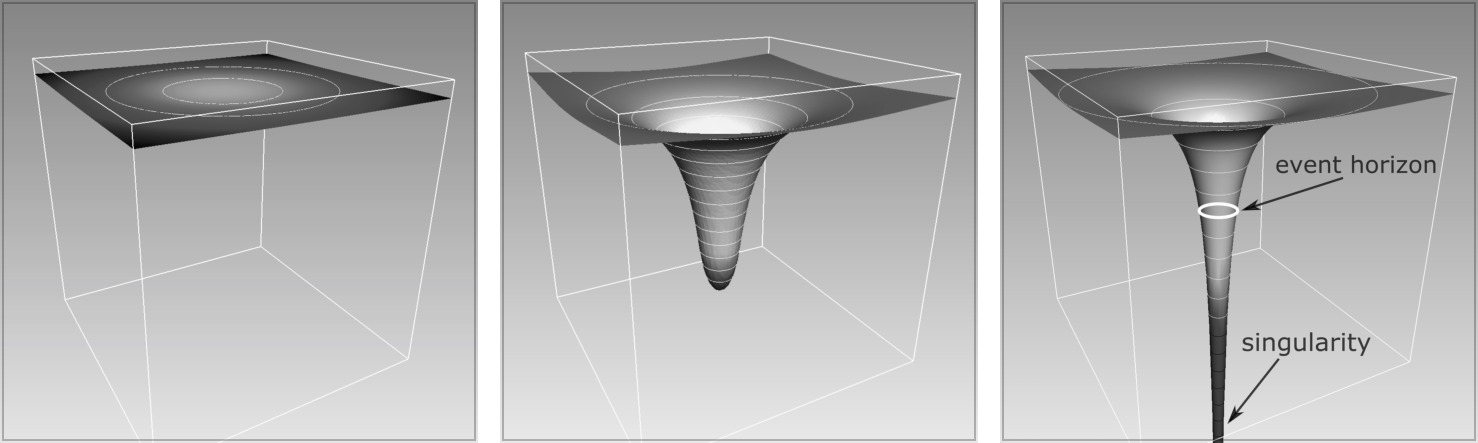
\includegraphics[width=0.88\linewidth,height=0.48\textheight,keepaspectratio]{../figs/pdf/en/fig-06-01.pdf}

% DOCX paragraph 733
\[\begin{array}{@{}w{c}{0.2933\linewidth}@{}w{c}{0.2933\linewidth}@{}w{c}{0.2933\linewidth}@{}}M/R\cong0{,}000002 & M/R\cong0{,}444 & M/R=0{,}5\end{array}\]

% DOCX paragraph 735
\caption{\emph{La curvatura del espaciotiempo producida por el Sol, a la izquierda, se genera al reducir su radio manteniendo su masa. El recuadro central representa el límite de Buchdahl, mientras que, en el de la derecha, su radio se ha reducido a solo 3 kilómetros, generando un agujero negro.}}\label{fig:06-01}
\end{figure}

% DOCX paragraph 737
Por último, el recuadro de la derecha muestra qué ocurriría si tomáramos la estrella ultracompacta\index{estrella ultracompacta} y la comprimiéramos aún más, aunque fuera muy poco, manteniendo siempre la misma masa. Obtendríamos un objeto con una superficie esférica de solo 3 kilómetros de radio y una compacidad de 0,5. ¡Es decir, un agujero negro! Al definir el radio de Schwarzschild\index{agujero negro!Schwarzschild} como el doble de la masa del agujero negro en la ecuación \eqref{eq:06-01}, también afirmamos implícitamente que la compacidad de un agujero negro de Schwarzschild es exactamente \emph{M/R=1/2=0,5}. En el tercer recuadro de la figura \ref{fig:06-01} he señalado la posición del horizonte de sucesos mediante una circunferencia de radio \emph{r=r\textsubscript{S}} (la superficie esférica aparece aquí como un círculo porque hemos suprimido una dimensión espacial). También se indica la posición de la singularidad física\index{singularidad!física}, situada en el centro de la «garganta\index{garganta}», es decir, en \emph{r=0}, y que por tanto no es visible en el recuadro.

% DOCX paragraph 738
Como ya estamos acostumbrados a hacer, podemos extraer una serie de consideraciones de la secuencia de la figura \ref{fig:06-01}. La primera es que el recuadro de la derecha, el del agujero negro, permite introducir una analogía mecánica para entender el papel de la gravedad y del horizonte de sucesos. Imagina que la superficie curva representa el fondo de un lago poco profundo con un agujero en el centro. El agujero creará una corriente que arrastrará el agua hacia el fondo, formando una enorme cascada (dejemos de lado por el momento la rotación, de manera que el agua no forme un remolino, sino que caiga siguiendo trayectorias radiales, como una cascada circular). Ahora imagina que estás en una embarcación con motores extraordinariamente potentes. Al acercarte a la cascada, la corriente aumenta, pero los motores tienen fuerza suficiente para avanzar contra ella y permiten que te acerques al borde del agujero e incluso lo sobrepases, aunque las paredes sean casi verticales. Pues bien, esto solo es posible hasta cierto punto. Habrá una «frontera» más allá de la cual los motores no podrán llevarte a contracorriente, por potentes que sean. Ni siquiera una potencia casi infinita sería suficiente. Para ti y para tu embarcación, ese límite representa, a todos los efectos, un «horizonte»: ¡una superficie que puedes atravesar, pero de la que no puedes salir!

% DOCX paragraph 739
La segunda consideración es que no hay soluciones intermedias entre el recuadro central y el de la derecha en la figura \ref{fig:06-01}. En otras palabras, si comprimimos, aunque sea infinitesimalmente, una estrella ultracompacta\index{estrella ultracompacta} que ha alcanzado el límite de Buchdahl, las ecuaciones de Einstein no permiten ninguna solución estática salvo la del agujero negro. En consecuencia, se crea una transición nítida entre las soluciones de objetos compuestos por materia y con superficie sólida, es decir, las estrellas compactas, y las que carecen de materia y de superficie sólida, es decir, los agujeros negros.

% DOCX paragraph 740
Una tercera consideración, al mirar la curvatura del último recuadro, es que parece que el espaciotiempo se haya «roto», como si su propia trama hubiese cedido bajo la acción irresistible de la gravedad. Pero en realidad el espaciotiempo no puede romperse, ya que es un continuo regular en todas partes, con la única excepción de la singularidad física\index{singularidad!física}. Deberíamos pensar, más bien, que un agujero negro lleva su elasticidad al máximo. Dicho de otro modo, aunque hemos visto que el espaciotiempo es en general bastante rígido, en el caso de un agujero negro la gravedad es tan fuerte que su deformabilidad alcanza el valor máximo.

% DOCX paragraph 741
Una cuarta consideración surge del hecho de que, al pasar de una estrella ultracompacta\index{estrella ultracompacta} a un agujero negro, hemos concentrado toda la materia en un único punto infinitesimal. Por tanto, un agujero negro está «vacío\index{vacío}», ya que toda la masa empleada para generarlo se concentra ahora en un punto de cero dimensiones. Se sigue que, a excepción de un punto en el centro, ¡el interior del horizonte de sucesos\index{horizonte de sucesos} está vacío! Así pues, las afirmaciones que sugieren la existencia de materia estable dentro de un agujero negro, de las que por desgracia se habla demasiado a menudo, son incorrectas. La densidad de materia en un agujero negro es exactamente \emph{cero}, porque un agujero negro es una solución de las ecuaciones de Einstein en el vacío.

% DOCX paragraph 742
Para concluir, déjame dedicar una última consideración al tiempo\index{caída libre!tiempo} que tarda en producirse un agujero negro. Creo que ya está claro que en física nada ocurre instantáneamente, y esto también se aplica al nacimiento de un agujero negro. Igual de claro está que, en relatividad general, ese tiempo depende inevitablemente de la posición y el movimiento del observador. Alguien que se encuentre lejos de un horizonte de sucesos nunca verá caer un objeto en él. Del mismo modo, alguien alejado de una estrella que colapsa nunca verá desaparecer su superficie bajo el horizonte. Verá, en cambio, una estrella que se contrae paulatinamente mientras emite una luz cada vez más débil y más desplazada al rojo, hasta que la radiación sea demasiado tenue para recibirla y la estrella desaparezca. Si el observador cayera junto con la materia que colapsa, la duración precisa del colapso\index{gravitatorio!colapso} dependería en parte de una serie de factores, como el tipo de materia o su rotación. Sin embargo, dejando de lado complicaciones innecesarias, desde el inicio del colapso, cuando la gravedad domina todas las demás interacciones físicas, el proceso tiene lugar esencialmente en el tiempo de caída libre. Es muy fácil calcular ese tiempo mediante una fórmula sencilla que sirve para cualquier objeto, grande o pequeño. Básicamente, la fórmula dice que el tiempo de caída libre es inversamente proporcional a la raíz cuadrada de la densidad del objeto que colapsa. Cuanto más denso sea, más breve será la caída libre. En el caso del Sol, nuestro ejemplo favorito, ese tiempo es de unos 27 minutos. Dicho de otra forma, si pudiéramos «apagar» por arte de magia todas las reacciones termonucleares de nuestra estrella y permitir que colapsara eliminando toda su presión interna, la superficie solar llegaría al centro en algo menos de media hora. Es un tiempo sorprendentemente breve si tenemos en cuenta que la materia de la superficie debe recorrer los 700\,000 kilómetros que la separan del centro del núcleo solar.

% DOCX paragraph 743
Todas estas consideraciones pretenden ayudarnos a imaginar lo que debió de ocurrir hace unos cinco millones de años, cuando la explosión de supernova\index{supernova} de una estrella muy masiva, de más de 40 masas solares, dio origen al agujero negro de Cyg X-1\index{Cyg X-1}. La diferencia más importante entre una supernova que da vida a una estrella de neutrones y otra que genera un agujero negro es que, en este último caso, el núcleo\index{hierro!núcleo} de hierro es mucho más masivo, del orden de unas diez masas solares. En estas condiciones, la densidad alcanzada durante el colapso\index{gravitatorio!colapso} es tal que ninguna presión, ni siquiera la de la materia degenerada que vimos en el capítulo 5, puede frenar el colapso final del núcleo estelar. Por tanto, cuando una cantidad suficiente de masa se concentra dentro de un radio del orden del radio de Schwarzschild, se produce inevitablemente un agujero negro.

% DOCX paragraph 744
Hoy en día, gracias a la solución numérica de las ecuaciones de Einstein y de la hidrodinámica\index{relativista!hidrodinámica} relativista, sabemos con bastante exactitud lo que sucede durante la formación de un agujero negro. En torno a 2005, junto con colegas europeos y estadounidenses, yo mismo estudié este proceso y obtuve las primeras simulaciones numéricas que lo describían en tres dimensiones, si bien partiendo de unas condiciones iniciales idealizadas. A pesar de estas simulaciones, muchos aspectos de la génesis astrofísica de los agujeros negros, tanto estelar\index{agujero negro!estelar}es como supermasivos, siguen sin estar claros. En el caso de los agujeros negros estelares, las observaciones electromagnéticas nos dicen que existen con masas de entre cinco y diez masas solares. En cambio, la detección de ondas gravitatorias\index{ondas gravitatorias} hasta el momento, de la que hablaremos en el capítulo 8, sugiere que los hay con masas de entre diez y 80 masas solares. La situación es aún más incierta cuando consideramos los agujeros negros supermasivos, es decir, de millones de masas solares o más. La incertidumbre es mucho mayor con respecto a la masa y a la era cosmológica en la que se producen por primera vez. No obstante, parece claro que incluso el nacimiento de estos enormes agujeros negros debe implicar, en algún momento, la concentración de cantidades ingentes de materia en una región de tamaño comparable al radio de Schwarzschild. Por esta razón, el experimento mental anterior sigue siendo perfectamente válido para todos los tipos de agujeros negros y constituye una referencia útil, sea cual sea la masa del agujero negro considerado.

% DOCX paragraph 747
\section{Los agujeros negros no tienen pelo}\label{sec:06-hair}

% DOCX paragraph 749
Hasta ahora he usado siempre la masa como única propiedad para distinguir entre los diversos tipos de agujeros negros, y me he referido a ellos como pequeños, o estelar\index{agujero negro!estelar}es, y grandes, o supermasivo\index{agujero negro!supermasivo}s. Pero es razonable preguntarse si un objeto tan complejo, descrito por ecuaciones extremadamente difíciles de manejar y aún más de resolver, puede realmente describirse solo en términos de su masa. En otras palabras, ha llegado el momento de preguntarnos: «¿Hasta qué punto son complejos los agujeros negros?».

% DOCX paragraph 750
Para responder, tengo que hacer una breve digresión. Desde pequeños, nuestra percepción\index{percepción} de la realidad, y por tanto nuestra comprensión del mundo, nos enseña que la complejidad va inevitablemente acompañada de una riqueza de detalles. Parece obvio que un fenómeno natural con una manifestación compleja debe estar lleno de «propiedades». Para que quede más claro, recurriré a unos ejemplos. Empecemos por un contexto que todos conocemos, al menos en términos generales: la música. Creo que resulta evidente que una sinfonía de música clásica interpretada por una gran orquesta es mucho más rica en contenido y, por tanto, en matices que el simple sonido de un diapasón. Como soy consciente de que hablar de «propiedades» o de «riqueza de contenido» puede resultar cualitativo y subjetivo, deberíamos optar por una medida más objetiva. Consideremos el número de instrumentos que intervienen en una sinfonía de duración media y multipliquémoslo por el número de notas musicales que se tocan durante la sinfonía. Obtendremos una medida mucho más cuantitativa y objetiva de su complejidad. Podemos hacer el mismo cálculo para un diapasón que repite su nota a intervalos regulares durante el mismo tiempo. En estos términos más objetivos, resulta trivial concluir que la orquesta sinfónica es cientos de veces más compleja que un diapasón.

% DOCX paragraph 751
Podemos encontrar ejemplos similares en un contexto biológico. Consideremos tres organismos vivos que nos resultan familiares: una bacteria como \emph{Escherichia coli}, una \emph{mosca Drosophila} y una \emph{lombriz}. Estos organismos se caracterizan por una complejidad creciente, ya que, en este orden, cada vez se necesita más información para describirlos. Para cuantificar esa complejidad, podemos fijarnos en su composición genética: 5\,000 genes para \emph{Escherichia coli}, 13\,000 para la \emph{mosca Drosophila} y 19\,000 para la lombriz (el número de genes de un ser humano es del orden de 30\,000). Como cada gen puede describirse mediante una combinación específica de aminoácidos, está claro que se necesita una enorme cantidad de información para describir incluso a los seres vivos más sencillos.

% DOCX paragraph 752
En esencia, tanto nuestra experiencia cotidiana como nuestro conocimiento del mundo sugieren que cuanto más complejo es un objeto, organismo o fenómeno físico, mayor es la cantidad de información necesaria para describirlo. Todo esto tendría sentido si no fuera porque los agujeros negros son una excepción llamativa a una regla muy razonable.

% DOCX paragraph 753
Basándonos en estos ejemplos, podríamos concluir que describir un agujero negro, el resultado más extremo de las ecuaciones más complejas de la física teórica, requeriría una enorme cantidad de información, y que la masa es solo una entre sus innumerables propiedades. Pues bien, sorprendentemente, no es así: ¡los agujeros negros son los objetos físicos macroscópicos más simples que existen! Esta conclusión se debe sencillamente a que, para describir cualquier agujero negro, solo necesitamos \emph{tres números}, que representan otras tantas propiedades. Una vez más, el concepto de agujero negro nos sorprende: es muchísimo más fácil de describir que la bacteria más elemental.

% DOCX paragraph 754
Entonces, ¿cuáles son esas tres, y solo tres, propiedades de un agujero negro? Son la masa\index{agujero negro!masa}, de la que ya hemos hablado; el \emph{espín\index{agujero negro!espín}}, es decir, la cantidad de rotación intrínseca; y, por último, la carga\index{agujero negro!carga} eléctrica. Por lo general, se representan mediante \emph{M} para la masa\index{agujero negro!masa}, \emph{J} para el momento angular de espín y \emph{Q} para la carga eléctrica. Así, podemos asignar a cualquier agujero negro un lugar en la «base de datos» del universo con solo darle los tres valores de \emph{M}, \emph{J} y \emph{Q}. En un escenario astrofísico realista, se espera que la carga eléctrica de un agujero negro sea prácticamente cero, de modo que podemos olvidarnos de ella. Es fácil entender por qué. Si alguna vez se generara un agujero negro con una carga eléctrica neta de cierto signo, las omnipresentes cargas libres, es decir, los electrones, protones y otras partículas cargadas que circulan por el espacio interestelar, algunas de las cuales tendrían necesariamente signo opuesto al de la carga del agujero negro, serían atraídas eléctricamente y absorbidas. Así, la carga del agujero negro disminuiría con rapidez hasta llegar a cero. En ese momento, el agujero negro sería eléctricamente neutro, es decir, \emph{Q=0}, y por tanto incapaz de atraer ninguna otra carga. Esto explica por qué, en la práctica, los astrofísicos solo emplean dos valores, \emph{M} y \emph{J}, para describir estos asombrosos cuerpos celestes.

% DOCX paragraph 755
El momento angular de espín debe estar dentro de un intervalo bien definido, lo que simplifica las cosas. Para expresarlo, conviene considerar cantidades \emph{adimensionales}, es decir, definidas de modo que no tengan dimensiones físicas (kilómetros, kilogramos, etc.) y sean, por tanto, números puros. Podemos definir el \emph{espín adimensional} del agujero negro como la razón entre su momento angular de espín y el cuadrado de su masa: \emph{a=J/M}\textsuperscript{2}. Pues bien, para un agujero negro en relatividad general, este número debe estar entre -1 y +1 (la diferencia de signo refleja la orientación de la rotación respecto a un eje de referencia y, por tanto, si el agujero negro gira en el sentido de las agujas del reloj o en sentido contrario). La cantidad \emph{a} es cero para un agujero negro de Schwarzschild\index{agujero negro!Schwarzschild}, que es, por tanto, un agujero negro \emph{sin rotación\index{agujero negro!sin rotación|see{agujero negro, Schwarzschild}}} (a partir de ahora me referiré a él como agujero negro \emph{de Schwarzschild} o \emph{sin rotación}). Si, en cambio, el espín adimensional \emph{a} es distinto de cero, hablaré de un agujero negro \emph{en rotación\index{agujero negro!en rotación|see{agujero negro, Kerr}}}, o agujero negro \emph{de Kerr\index{agujero negro!Kerr}}, en honor al matemático neozelandés Roy Kerr, el primero que encontró esta solución\textsuperscript{\hyperlink{note:06-04}{4}}. Como los agujeros negros suelen acretar materia con cierta cantidad de momento angular, en un contexto astrofísico se espera que sean siempre del tipo Kerr, aunque algunos roten muy despacio.

% DOCX paragraph 756
La peculiar conclusión de que solo tres propiedades describen un agujero negro está contenida en el famoso «\emph{teorema de ausencia de pelo\index{agujero negro!pelo}}». Este nombre humorístico, acuñado por el ya mencionado John Wheeler y por el astrofísico italiano Remo Ruffini\index{Ruffini, Remo}\textsuperscript{\hyperlink{note:06-05}{5}}, pretende subrayar que, si vemos un agujero negro como una esfera, carece de detalles, igual que una cabeza puede carecer de pelo. La tesis del teorema, muy sencilla de formular, afirma esencialmente que, en relatividad general, un agujero negro aislado y situado en un espaciotiempo asintóticamente plano, es decir, que se vuelve plano a grandes distancias, puede describirse mediante esos tres valores: \emph{M}, \emph{J} y \emph{Q}. Curiosamente, si algo modifica uno de ellos, por ejemplo la caída de materia con momento angular que cambia los valores de \emph{M} y \emph{J}, a la variación de los parámetros le sigue un estado en el que desaparecen todas las perturbaciones transitorias y queda un «nuevo» agujero negro. Aunque distinto del anterior, sigue estando descrito por los valores \emph{M}, \emph{J} y \emph{Q} (volveremos a este punto en el capítulo 8).

% DOCX paragraph 759
\section{Motores cósmicos y radiación de Hawking}\label{sec:06-hawking}

% DOCX paragraph 761
En muchos sentidos, los agujeros negros pueden verse como «\emph{motores cósmicos}» capaces de absorber materia del exterior y modificar así su masa, su momento angular y su carga eléctrica (véase la figura \ref{fig:06-02}). Existen tres leyes de la «dinámica de los agujeros negros» que nos dicen cómo pueden cambiar con el tiempo las propiedades \emph{M}, \emph{J} y \emph{Q} mediante la interacción con el mundo exterior. Dejando de lado la carga \emph{Q}, cuya evolución ya hemos comentado, estas leyes, que se derivan de la relatividad general\index{relatividad general} clásica sin tener en cuenta los efectos de la mecánica cuántica, nos dicen que la masa de un agujero negro solo puede aumentar. En cambio, su momento angular puede aumentar o disminuir, hasta llegar a cero. En esencia, un agujero negro en rotación puede ralentizarse y convertirse en uno sin rotación al perder su energía rotacional. Cuando esto ocurre, una parte de la masa del agujero negro puede reducirse, pero no toda su masa. Más precisamente, la parte de la masa asociada a la rotación, la que depende de \emph{J}, puede disminuir; por razones obvias, se llama \emph{masa reducible\index{agujero negro!masa reducible}\index{masa!reducible}}. Sin embargo, hay una parte de la masa que no está ligada a la rotación, es decir, que no depende de \emph{J}, y que no puede disminuir, sino solo aumentar. También por razones obvias, esta parte recibe el nombre de \emph{masa irreducible\index{agujero negro!masa irreducible}\index{masa!irreducible}}.

% DOCX paragraph 762
La ley según la cual un agujero negro no puede perder su masa irreducible, en la formulación clásica de la relatividad general, fue revolucionada en los años setenta por el físico británico Stephen\index{Hawking!Stephen} Hawking. Propuso un nuevo mecanismo relacionado con los principios de la mecánica cuántica\index{mecánica cuántica} que, en efecto, viola esa ley.

% DOCX paragraph 764
\begin{figure}[htbp]
\centering
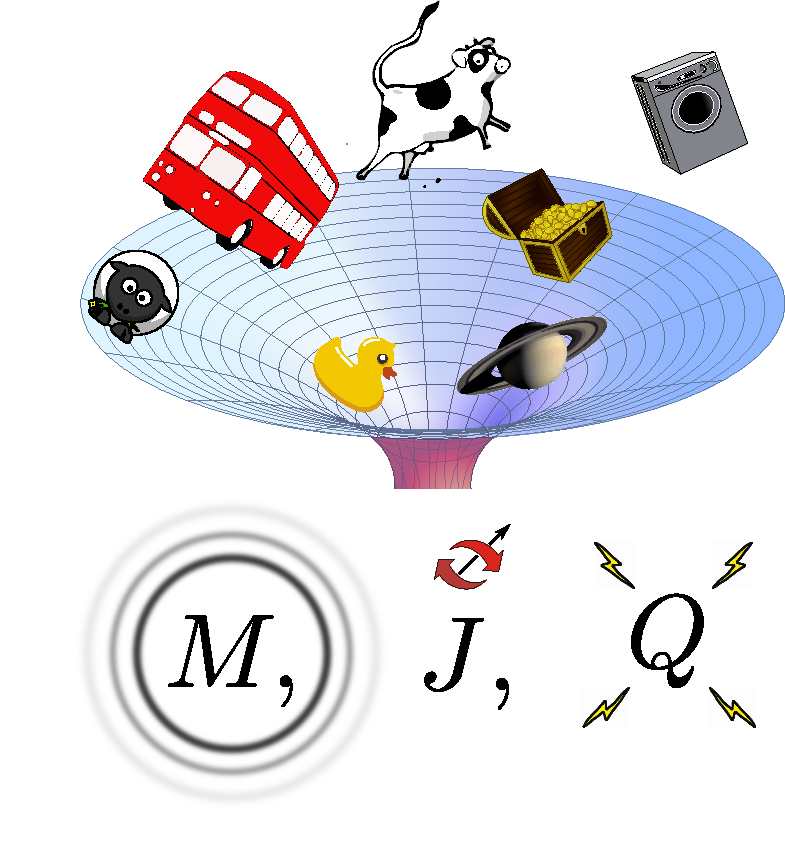
\includegraphics[width=0.88\linewidth,height=0.48\textheight,keepaspectratio]{../figs/pdf/en/fig-06-02.pdf}

% DOCX paragraph 765
\caption{Teorema de ausencia de pelo\emph{: sea cual sea el tipo de objetos que absorban los agujeros negros, estos solo producen un cambio en los tres números que caracterizan a un agujero negro\index{agujero negro!espín}: la masa\index{agujero negro!masa} M, el momento angular J y la carga\index{agujero negro!carga} eléctrica Q.}}\label{fig:06-02}
\end{figure}

% DOCX paragraph 767
Hawking\index{radiación!Hawking} sugirió que un agujero negro podía «evaporarse» y, por tanto, perder masa, tanto reducible como irreducible, mediante la emisión de una radiación\index{Hawking!radiación} térmica llamada \emph{radiación de Hawking}\textsuperscript{\hyperlink{note:06-06}{6}}. Para producirla, es necesario generar una serie de partículas y antipartículas virtuales, es decir, partículas con «masa/energía negativa\index{energia@energía!negativa}», en una región extremadamente delgada cerca del horizonte de sucesos. Sabemos que las partículas y las antipartículas pueden producirse en cualquier lugar del espaciotiempo, sin ningún efecto neto, ya que el número de antipartículas virtuales producidas se equilibra exactamente con el de las partículas correspondientes. Sin embargo, cuando el fenómeno ocurre cerca de un horizonte de sucesos, que solo puede absorber partículas, pero no emitirlas, es posible un resultado neto: el efecto global es que el agujero negro emite radiación en forma de esas partículas virtuales. Al mismo tiempo, su masa disminuye debido a la acreción de antipartículas, que tienen masa-energía negativa y, por tanto, contribuyen con una masa negativa.

% DOCX paragraph 768
No hay pruebas experimentales de la existencia de la radiación de Hawking\index{radiación!Hawking}\index{luminosidad!Hawking}. La razón principal, por supuesto, es que resulta imposible crear un agujero negro en el laboratorio, aunque en principio sea posible generar objetos con propiedades similares, llamados «análogos» de agujero negro. Pero no es la única razón: la radiación de Hawking es muy débil para los agujeros negros estelar\index{agujero negro!estelar}\index{agujero negro!estelar}es, y aún más para los supermasivos. Más precisamente, la \emph{luminosidad\index{Hawking!luminosidad} de Hawking}, es decir, la cantidad de masa-energía que pierde un agujero negro por unidad de tiempo debido a esta radiación, es inversamente proporcional al cuadrado de su masa. Por tanto, incluso un agujero negro «ligero», de una masa solar, tardaría unos 10\textsuperscript{67} años en evaporarse por completo. Si tenemos en cuenta que el universo tiene unos 10\textsuperscript{10} años, está claro que un agujero negro de esa masa tardaría en evaporarse miles de millones y miles de millones y miles de millones y miles de millones de veces la edad del universo. Los tiempos son aún mayores para agujeros negros más masivos, como el que hay en el centro de nuestra galaxia. Por eso, la mejor oportunidad de observar la radiación de Hawking la ofrecen los agujeros negros extremadamente pequeños. En particular, un agujero negro que se hubiera generado en el universo primitivo con una masa de 10\textsuperscript{11} kilogramos, es decir, una milmillonésima parte de la de un asteroide, emitiría suficiente radiación de Hawking para estar a punto de evaporarse.

% DOCX paragraph 769
A pesar de esta falta de pruebas observacionales, la comunidad científica coincide en que la radiación de Hawking\index{radiación!Hawking} es físicamente posible y en que, al menos en principio, un agujero negro también puede perder masa, hasta desaparecer por completo o dejar una singularidad muy pequeña.

% DOCX paragraph 770
En resumen, cuando hablamos de masa, los agujeros negros parecen comportarse como los humanos: a veces pueden «perder peso» si bajan el ritmo, pero en la inmensa mayoría de los casos, tarde o temprano, tienden inevitablemente a engordar~...

% DOCX paragraph 773
\section{Una idea difícil de digerir}\label{sec:06-idea}

% DOCX paragraph 775
La «ausencia de pelo» en los agujeros negros nos invita a reflexionar sobre por qué la propia idea de estos objetos, y en particular la existencia de un horizonte de sucesos\index{horizonte de sucesos}, sigue siendo difícil de aceptar. Un horizonte de sucesos hace que el agujero negro sea decididamente «\emph{excepcional}», en el sentido de que representa una \emph{excepción} a lo que sabemos y estamos acostumbrados a aceptar en física. Una vez cruzada la superficie matemática del horizonte de sucesos, toda la información sobre las propiedades del objeto que entra en el agujero negro se pierde, convertida, junto con toda su complejidad, en las únicas tres propiedades que un observador externo puede medir: \emph{M}, \emph{J} y \emph{Q}.

% DOCX paragraph 776
Si lo piensas, este comportamiento es, como mínimo, anómalo, y desde luego no es lo que estamos acostumbrados a ver en física. Déjame darte un ejemplo que ilustra hasta qué punto es excepcional. Imagina que tomas unos troncos y enciendes una buena hoguera; cuando las llamas se apagan, de la madera solo quedan unas cenizas finas e indistinguibles. Tal vez no pensarías que esas cenizas contienen información sobre las propiedades originales de la madera o las propiedades químicas de las células orgánicas que la constituían. En esencia, creerías imposible recuperar algún rastro que permitiera establecer si los troncos procedían de un haya o de un roble. ¡Toda la información parecería haberse esfumado!~... Pues bien, ¡ahí está precisamente la cuestión! Las cenizas no son el único producto del fuego, y es posible, al menos en principio, reconstruir las propiedades de la madera estudiando los gases del humo producido durante la combustión.

% DOCX paragraph 777
Este ejemplo muestra que, aunque los sistemas físicos pueden sufrir transformaciones, la información completa sobre sus propiedades nunca se pierde. Por supuesto, esas propiedades pueden cambiar, y de hecho cambian, y es muy posible que cada vez resulte más difícil reunir información sobre ellas: basta pensar en el humo. Sin embargo, por razones que están en el corazón mismo de nuestra comprensión de la física, la información sobre el sistema nunca se pierde. ¡La única excepción a esta lógica elemental es lo que ocurre con un agujero negro! Solo en este caso perdemos toda la información sobre las propiedades de aquello que generó su masa, su momento angular y su carga, aunque disponíamos de ella hasta el momento en que se cruzó el horizonte de sucesos.

% DOCX paragraph 778
La imposibilidad de extraer información de un agujero negro se conoce como \emph{paradoja de la pérdida de información\index{paradoja de la pérdida de información}}, y es mucho más grave de lo que puede parecer. De hecho, socava los fundamentos mismos de la mecánica cuántica\index{mecánica cuántica}, según la cual la información de un sistema físico no puede perderse. Más precisamente, la paradoja surge porque, al describir el estado de un sistema mediante una función de onda, la evolución de esa función debe ser unitaria (recordemos que un postulado fundamental de la mecánica cuántica establece precisamente que toda la información de un sistema físico está contenida en su función de onda). Dicho de otro modo, una vez especificadas las condiciones iniciales de la función de onda del sistema, su evolución queda completamente determinada. Sin embargo, en un agujero negro se viola esta unitariedad, de modo que varios estados inicialmente distintos se fusionarían en uno solo y se volverían indistinguibles.

% DOCX paragraph 779
La paradoja de la pérdida de información sigue sin resolverse, a pesar de décadas de estudios. Ninguna de las teorías propuestas para eliminarla resulta lo bastante convincente como para ser aceptada: una nueva y clamorosa confirmación de la incompatibilidad entre la relatividad general clásica, tal como la formuló Einstein, y los principios de la mecánica cuántica\index{mecánica cuántica}.

% DOCX paragraph 782
\section{Renunciar a un método querido}\label{sec:06-method}

% DOCX paragraph 784
Hay otro aspecto que hace del horizonte de sucesos un concepto bastante «indigesto» para los físicos. Si recuerdas, en el capítulo 2 insistí en la importancia de la obra de Galileo al definir e introducir el método científico\index{método científico}, el único faro que ilumina las especulaciones humanas. A lo largo de los siglos, su trabajo nos ha permitido alcanzar conclusiones firmes en los debates, algunos de siglos de duración, que inevitablemente caracterizan la exploración científica: qué es verdadero y qué es falso, qué es correcto y qué es erróneo. El propio Galileo resumió la importancia del método en uno de sus aforismos más conocidos. Dirigiéndose a Tommaso Campanella, declaró: «Prefiero encontrar una verdad, aunque sea en una cosa pequeña, a discutir sobre las mayores cuestiones sin obtener ninguna verdad». En el caso de un agujero negro, es imposible encontrar una sola verdad, al menos en los términos del método científico, sobre lo que hay más allá del horizonte de sucesos. ¡Y no porque las leyes de la física dejen de ser válidas!

% DOCX paragraph 785
Intentaré explicar mejor a qué me refiero. Imagina a dos observadores fuera de un agujero negro supermasivo: Simplicio\index{Simplicio} y Salviati\index{Salviati}\textsuperscript{\hyperlink{note:06-07}{7}}. Discuten sobre si es posible realizar un experimento dentro del horizonte de sucesos\index{horizonte de sucesos}. Aplicando su propia lógica, Simplicio, que no es un experto en relatividad general, afirma que, tras cruzar el horizonte, hay un mundo fantástico en el que no se puede hacer ningún experimento. En cambio, cualquiera puede obtener lo que desee con solo pensarlo. Según Simplicio, si cruzara ese límite encontraría una mesa repleta de alimentos deliciosos y, en particular, su helado favorito (a Simplicio le encanta comer, y todos saben que no puede resistirse al helado).

% DOCX paragraph 786
Para Salviati\index{Salviati}, que conoce bien la relatividad general, nada de esto ocurre dentro del horizonte de sucesos de un agujero negro supermasivo. Las leyes de la física\index{singularidad!física} siguen siendo válidas allí, y cualquier objeto que haya entrado debe acabar en la singularidad física, sobre la cual, admite, no puede hacer ninguna predicción. Salviati también sostiene que, si la masa del agujero negro es muy grande, un objeto del tamaño de un ser humano experimentará fuerzas de marea\index{fuerzas de marea} muy pequeñas y no notará ningún cambio apreciable al cruzar el horizonte de sucesos. Excepto, naturalmente, que ya no podrá comunicarse con el mundo exterior.

% DOCX paragraph 787
A la luz de lo que sabemos de física, todos podemos coincidir en que la tesis de Simplicio\index{Simplicio} está cogida por los pelos. No tiene ningún apoyo lógico ni científico, y no hay motivos para creer que sea correcta. Pero ese es precisamente el problema: la discusión entre los dos no puede resolverse, aunque se trate de «una cosa pequeña», en palabras de Galileo. La razón es sencilla: ni Salviati\index{Salviati} ni nadie puede entrar en el horizonte de sucesos, comprobar que no hay mesas repletas de alimentos deliciosos e informar del resultado al resto del mundo. Lo que aún irrita más a Salviati es que sabe muy bien que sería posible \emph{realizar} un experimento que refutase la tesis de Simplicio. El problema sería comunicar los resultados al exterior, algo imposible una vez dentro del horizonte de sucesos.

% DOCX paragraph 788
Aceptar la existencia de un horizonte de sucesos equivale, por tanto, a admitir que en nuestro universo hay regiones físicamente accesibles que quedan fuera del alcance de una investigación basada en el método científico\index{método científico}. No es porque la física deje de ser válida allí, ya que, al menos en relatividad general, la única región problemática es un punto infinitesimal en el centro del agujero negro. El problema es mucho más sencillo: los resultados de los experimentos realizados dentro del horizonte de sucesos no pueden darse a conocer. Una perspectiva que sin duda haría que el pobre Galileo se revolviera en su tumba~...

% DOCX paragraph 789
Podemos recurrir aquí a una analogía un tanto arriesgada. El horizonte de sucesos\index{horizonte de sucesos} plantea las mismas complicaciones conceptuales e implicaciones filosóficas que la vida después de la muerte: algo en lo que muchos creen, pero que nadie puede demostrar porque, salvo conocidas excepciones, nadie ha regresado para contarnos qué hay después de morir.

% DOCX paragraph 790
Estas consideraciones muestran por qué la idea de un horizonte de sucesos resulta tan difícil de digerir para los físicos, que, por aspiración o ambición, queremos extender el conocimiento a todos los rincones del universo. Para nosotros, el horizonte de sucesos es como una puerta que puede abrirse y atravesarse, pero que luego se cierra para siempre a nuestra espalda. Por eso, a lo largo de los años, y en particular durante la última década, se ha dedicado un considerable esfuerzo intelectual a estudiar los llamados \emph{imitador\index{agujero negro!imitador}es de agujeros negros}. Son objetos con los que intentamos mitigar algunas de las dificultades conceptuales que plantean los agujeros negros, y que examinaremos con más detalle en la siguiente sección.

% DOCX paragraph 793
\section{Observaciones frente a experimentos}\label{sec:06-observations}

% DOCX paragraph 795
Hemos visto que la presencia de un horizonte de sucesos y de una singularidad física\index{singularidad!física} en el centro hace que la propia idea de agujero negro resulte difícil de digerir. Ante estas dificultades, podrías preguntarte: «¿Es posible prescindir de los agujeros negros?».

% DOCX paragraph 796
Muchos se han enfrentado a esta pregunta, sobre todo en los últimos años, con las observaciones directas de objetos compatibles con agujeros negros, tanto a través de la detección de ondas gravitatorias por la colaboración LIGO\index{LIGO}/Virgo como gracias a la primera «fotografía» de un agujero negro, obtenida por la colaboración Event Horizon Telescope, o EHT\index{EHT (Event Horizon Telescope)}.

% DOCX paragraph 797
Antes de responder, es necesario hacer una consideración más general sobre cómo progresa el conocimiento científico, sobre todo en astrofísica.

% DOCX paragraph 798
La astrofísica, la única rama de la física que aporta pruebas de la existencia de agujeros negros, es una ciencia\index{observacional!ciencia}\index{experimental!ciencia} \emph{observacional\index{ciencia!observacional}}, no \emph{experimental\index{ciencia!experimental}}. A diferencia de ramas como la física del estado sólido o la de partículas elementales, en ella no es posible realizar experimentos. Dicho de otro modo, en astrofísica no podemos construir un dispositivo experimental que permita producir, de manera controlada, las condiciones físicas en las que se espera que ocurra un determinado fenómeno. Con «de manera controlada» me refiero a la posibilidad de realizar un experimento teniendo una idea clara de los errores que pueden afectar a las medidas. La astrofísica, en cambio, debe recurrir a las observaciones astronómicas para formular teorías que después puedan confirmarse o refutarse mediante nuevas observaciones. Este aspecto, que a veces se pasa por alto o incluso se ignora, añade una considerable complejidad a la aplicación del método científico por al menos dos razones.

% DOCX paragraph 799
La primera es que, al disponer solo de observaciones, suele ser difícil predecir el número de fuentes que se estudiarán y sus propiedades. A modo de comparación, cuando se construye un acelerador de partículas como el del CERN\index{CERN}, una vez fijadas las condiciones iniciales, por ejemplo la energía del haz incidente o las propiedades del haz que sirve de blanco, se tiene una idea exacta del número de sucesos o colisiones que pueden producirse en un tiempo determinado. Por desgracia, en astrofísica no es tan sencillo: salvo que se pretenda repetir observaciones de fuentes bien conocidas, la construcción de un telescopio suele ir acompañada de una gran incertidumbre sobre el número de objetos nuevos que se observarán. Por ejemplo, cuando entraron en funcionamiento los detectores de ondas gravitatorias de la colaboración LIGO\index{LIGO} (no olvidemos que la astronomía de ondas gravitatorias también es una ciencia observacional), la incertidumbre sobre el número de sucesos que podrían medirse era de tres órdenes de magnitud. En otras palabras, no se sabía si habría 400 sucesos al año o solo 0,4.

% DOCX paragraph 800
La segunda razón por la que el progreso científico es más difícil en astrofísica es que, al ser una ciencia observacional, sufre una \emph{degeneración\index{degeneración!interpretación}} entre las posibles explicaciones de las observaciones. Recurriré de nuevo a una analogía. Imagina un antiguo reloj de pared que puedes observar cuanto quieras. ¿Qué notarías? Probablemente que tiene dos agujas, una larga y otra corta, y que la corta gira 360 grados cada 12 horas, mientras que la larga hace lo mismo cada 60 minutos. Estas son tus «observaciones». Supón ahora que debes construir un modelo matemáticamente completo y físicamente plausible del mecanismo interno que hace funcionar el reloj. Como puedes imaginar, encontrarías muchos modelos matemáticos y combinaciones de mecanismos que explicasen perfectamente la vuelta de la aguja larga cada 60 minutos y la de la corta cada 12 horas. Sin embargo, solo una de esas explicaciones es la correcta, y es posible que ni siquiera la hayas considerado. Para remediar esta dificultad, tendrías que emplear toda tu imaginación e ingenio en obtener información adicional. Podrías, por ejemplo, utilizar micrófonos para escuchar el ruido\index{ruido} del mecanismo que produce el movimiento y servirte de las grabaciones para descartar modelos incompatibles con las «observaciones acústicas». O medir las vibraciones que el reloj transmite a la pared y trabajar en modelos compatibles con esa nueva información.\index{señal|see{ruido}}

% DOCX paragraph 801
Pues bien, la astrofísica progresa de un modo parecido. También aquí toda la información disponible se recoge únicamente mediante observaciones, que los científicos intentan explicar con modelos matemáticos construidos a partir de las leyes de la física. La información adicional puede proceder de observaciones en distintas bandas electromagnéticas o en distintos canales de observación, en cuyo caso hablamos, respectivamente, de \emph{astronomía multibanda\index{astronomía!multibanda}\index{astronomía multibanda}} o \emph{multimensajero\index{astronomía!multimensajero (ondas gravitatorias)}\index{astronomía!multimensajero}}. Como ocurre con el reloj de pared, incluso los modelos que parecen más exactos y ofrecen explicaciones más plausibles pueden resultar incorrectos, precisamente porque hay una degeneración\index{degeneración!interpretación} entre las observaciones y los modelos capaces de explicarlas. La creatividad de los astrofísicos les permite utilizar todas las observaciones posibles, y las conexiones entre ellas, para reducir el conjunto de modelos compatibles con los datos o predecir comportamientos cuya observación, o ausencia, pueda confirmar o refutar el modelo.\index{astronomía multimensajero}

% DOCX paragraph 804
\section{Imitadores de agujeros negros}\label{sec:06-mimickers}

% DOCX paragraph 806
Volvamos a los imitador\index{agujero negro!imitador}es de agujeros negros. Nuestra digresión sobre los aspectos epistemológicos de la astrofísica\index{singularidad!física} ha servido para mostrar que, aunque la solución del agujero negro sea la explicación más natural y sencilla de la fenomenología observada en objetos astrofísicos compactos como Cyg-X1, no es la única. Hay otras explicaciones que no requieren un agujero negro. Es fácil adivinar las características de estas soluciones alternativas: representan objetos extremadamente compactos, sin horizonte de sucesos ni singularidad física\textsuperscript{\hyperlink{note:06-08}{8}}. De hecho, la relatividad general\index{relatividad general} y varias «\emph{teorías alternativas\index{teorías alternativas (gravedad)}}» de la gravedad permiten la existencia de toda una clase de objetos astrofísicos compactos con estas propiedades, por lo que reciben el nombre de «\emph{imitadores}» de agujeros negros. Sus propiedades se parecen tanto a las de estos que a veces resultan casi indistinguibles, al menos en las medidas realizadas por observadores lejanos como nosotros.

% DOCX paragraph 807
Examinemos algunos de estos imitadores. En primer lugar, la llamada \emph{estrella\index{gravitatoria!estrella (véase gravastar)} gravitatoria}, o simplemente \emph{gravastar\index{gravastar}}. Se trata de una solución de las ecuaciones de Einstein con simetría esférica\index{simetría esférica}, perfectamente compatible, por tanto, con lo que sabemos de relatividad general, que propusieron en 2000 los físicos Pawel Mazur\index{Mazur, Pawel} y Emil Mottola\index{Mottola, Emil}\textsuperscript{\hyperlink{note:06-09}{9}}. La solución supone una estrella formada por capas, con un núcleo interno que ocupa casi toda la estrella y está compuesto de materia de propiedades muy poco habituales: a diferencia de todo aquello a lo que estamos acostumbrados, tiene presión negativa\index{presión!negativa} (toda la materia que conocemos tiene presión positiva\index{presión!positiva}). Este núcleo está rodeado por una «piel» muy delgada de materia con propiedades igualmente extremas: una presión extraordinariamente alta, pero positiva.\index{exótico!objeto compacto (gravastar)}

% DOCX paragraph 808
La materia con presión negativa puede considerarse como un pequeño universo que quiere expandirse y está asociada a un «espaciotiempo\index{de Sitter!espaciotiempo} de de Sitter», por el científico neerlandés Willem\index{de Sitter!Willem} de Sitter, el primero que lo propuso. De hecho, creemos que esta solución de las ecuaciones de Einstein está relacionada con la expansión acelerada que medimos actualmente en cosmología. Al mismo tiempo, la delgada capa de materia a muy alta presión situada en la superficie de la gravastar\index{gravastar} quiere colapsar, lo que contrarresta la expansión del núcleo y genera un equilibrio estable. Dicho de otro modo, ¡una gravastar es como un globo con presión interna negativa, pero con un gradiente positivo hacia fuera! Su delgada superficie exterior impide que el núcleo se expanda.

% DOCX paragraph 809
La peculiaridad más importante de esta solución es que puede construirse de modo que tenga una compacidad muy cercana a la de un agujero negro, apenas por debajo de ella, es decir, \emph{M/R} \(\lesssim \ 1/2\). En particular, es posible construir, al menos como soluciones matemáticas, gravastar\index{compacidad!gravastar}\index{gravastar}s cuya superficie esté justo por encima de donde estaría el horizonte de sucesos\index{horizonte de sucesos} de un agujero negro de la misma masa, con un radio solo infinitesimalmente mayor que el de un agujero negro de Schwarzschild\index{agujero negro!Schwarzschild}. Por tanto, las gravastars tienen una superficie rígida, como las estrellas de neutrones (de ahí el nombre de «estrella» gravitatoria), pero carecen de horizonte de sucesos y de singularidad física\index{singularidad!física} en \emph{r=0}: son soluciones perfectamente regulares.

% DOCX paragraph 810
El segundo ejemplo de imitador de agujero negro se ha convertido casi en un «clásico»: el \emph{agujero de gusano}. Como en el caso del agujero negro, este nombre evocador también lo acuñó John Wheeler, en un artículo escrito con Charles Misner en 1957\textsuperscript{\hyperlink{note:06-10}{10}}.

% DOCX paragraph 811
Se trata, una vez más, de una solución perfectamente plausible de las ecuaciones de Einstein para un objeto en el vacío\index{vacío} y extremadamente compacto, aunque con una compacidad ligeramente menor que la de un agujero negro. Lo interesante es que, gracias a la gran curvatura que producen los agujeros de gusano, en principio es posible unir dos regiones del espaciotiempo muy distantes y asintóticamente planas. En esencia, la solución del agujero de gusano\index{compacidad!agujero de gusano} puede verse como un túnel en la trama elástica del espaciotiempo, un «atajo» entre dos regiones físicamente alejadas. Imagina que tomas una sección de espaciotiempo plano de dos dimensiones, nuestra querida sábana del capítulo 3, y consideras dos puntos muy alejados entre sí. Si doblas un extremo de la sábana hasta obtener dos capas paralelas, los puntos ya no estarán tan lejos: bastaría poder viajar \emph{a través} de la sábana en lugar de hacerlo a lo largo de ella. Ahora imagina una fuente de gravedad lo bastante intensa como para deformarla y crear una doble garganta\index{garganta}. Ya está: has creado un atajo entre los dos puntos, antes lejanos y ahora muy próximos. Hace tiempo que se demostró que los agujeros de gusano, al menos en los modelos más sencillos, son dinámicamente inestables: si se abrieran, tenderían a cerrarse con extrema rapidez. Al mismo tiempo, existen soluciones de agujeros de gusano que pueden estabilizarse mediante la presencia en la garganta de materia\index{exótica!materia} exótica, es decir, con masa o energía negativa\index{energia@energía!negativa}s.

% DOCX paragraph 813
\begin{figure}[htbp]
\centering
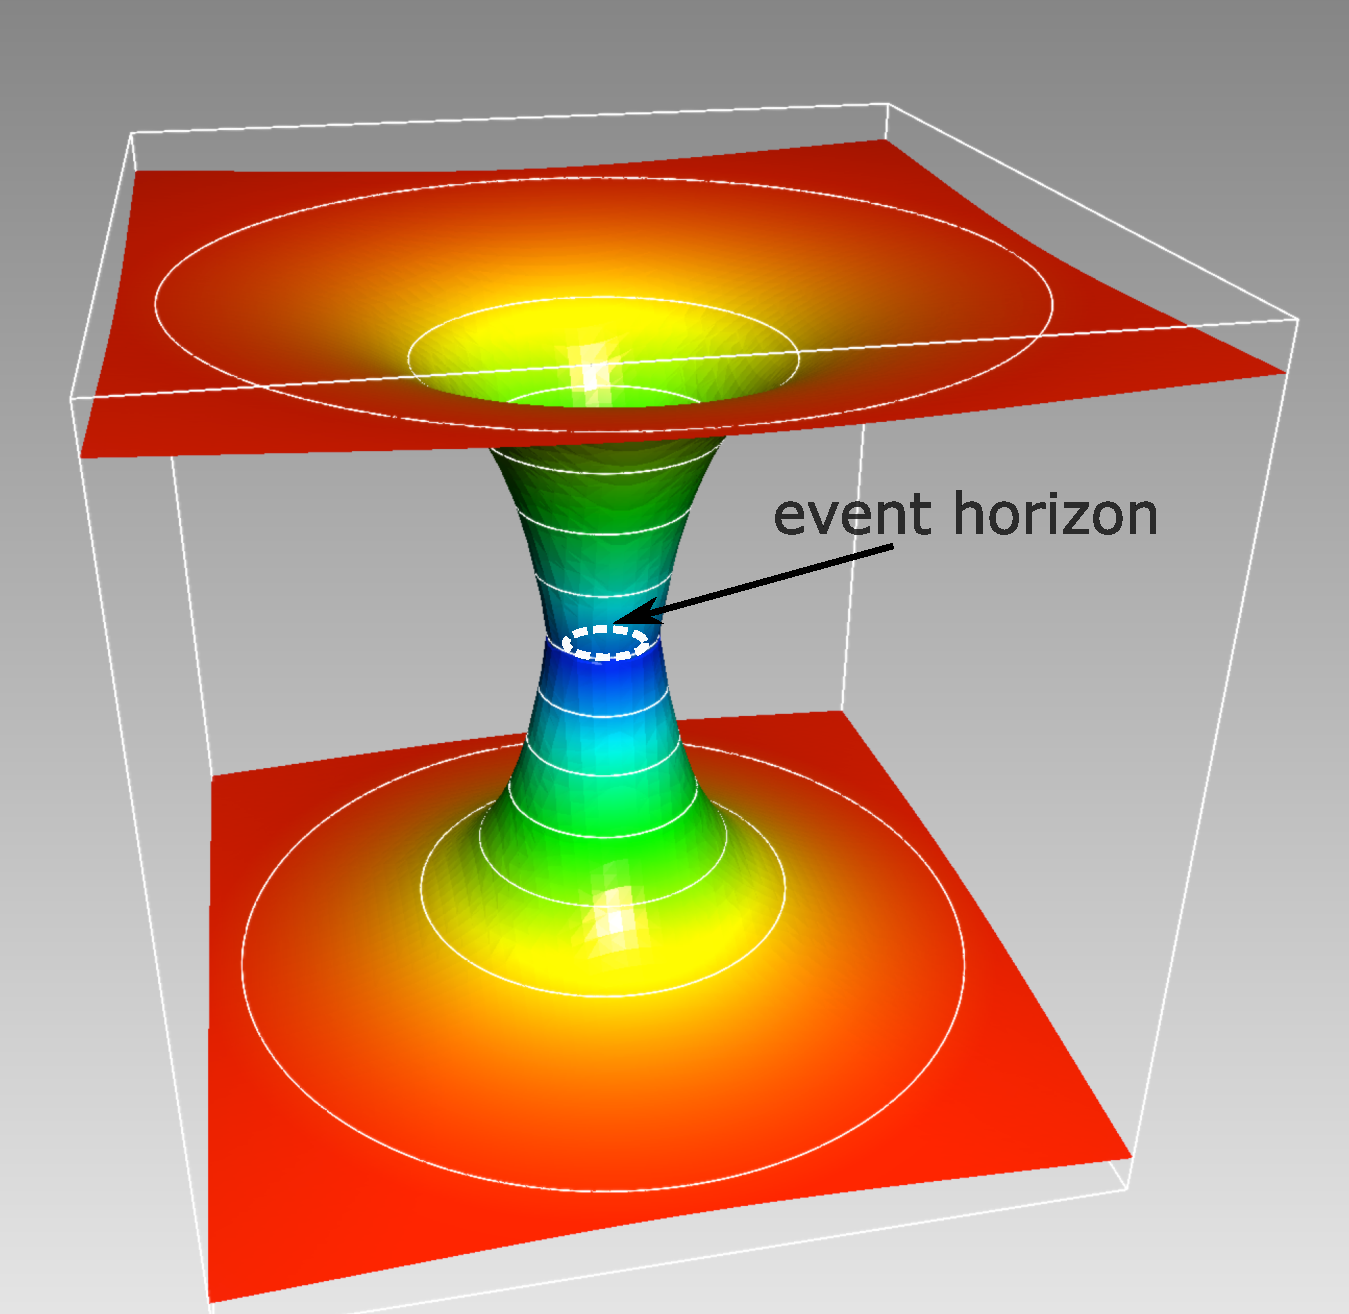
\includegraphics[width=0.88\linewidth,height=0.48\textheight,keepaspectratio]{../figs/pdf/en/fig-06-03.pdf}

% DOCX paragraph 815
\caption{\emph{Los agujeros de gusano con dos «garganta\index{garganta}s» idénticas y simétricas pueden unir dos regiones del espaciotiempo planas a grandes distancias. La sección más estrecha de la garganta es ligeramente mayor que la de un agujero negro de Schwarzschild\index{agujero negro!Schwarzschild} de la misma masa.}}\label{fig:06-03}
\end{figure}

% DOCX paragraph 817
El esquema de un agujero de gusano de la figura \ref{fig:06-03} muestra la «garganta\index{garganta}» típica a la que nos hemos acostumbrado cuando hay una curvatura intensa. Sin embargo, en este caso las dos gargantas son exactamente simétricas y pueden unir dos regiones del espaciotiempo\index{espaciotiempo!plano} planas a grandes distancias. Aun así, conviene señalar que también aquí la sección más estrecha de la garganta es ligeramente mayor que la que tendría un agujero negro de Schwarzschild\index{agujero negro!Schwarzschild} de la misma masa, como indica el círculo blanco discontinuo. Por tanto, no se trata de un agujero negro, sino de un objeto muy compacto.

% DOCX paragraph 818
Una gravastar y un agujero de gusano difieren considerablemente en al menos un aspecto: la primera tiene una superficie sólida, como una estrella de neutrones, mientras que el segundo carece de ella y, al menos en los modelos más sencillos, es una solución en el vacío\index{vacío}. Al mismo tiempo, tienen al menos dos propiedades en común. En primer lugar, ambos poseen una compacidad \emph{M/R} extremadamente alta, muy próxima a la de un agujero negro, \emph{1/2}, aunque algo menor. La segunda propiedad común es su «génesis». En ambos casos, solo tenemos una idea vaga de cómo podrían producirse estos objetos en la naturaleza. Dicho de otro modo, aunque las gravastars y los agujeros de gusano son soluciones admisibles y perfectamente legítimas de las ecuaciones de Einstein, al menos por ahora no conocemos los procesos astrofísicos que podrían dar lugar a su formación. La situación es muy distinta para objetos igualmente compactos, como las estrellas de neutrones o los agujeros negros. Hemos identificado trayectorias evolutivas precisas que permiten partir de estrellas de entre 10 y 100 masas solares y llegar, a través de una evolución descrita en detalle por la astrofísica nuclear, a una supernova\index{supernova} y, por tanto, a la formación de una estrella de neutrones o de un agujero negro, según la masa de la estrella original. Sin embargo, ni siquiera con lo que hoy sabemos de astrofísica nuclear y de los procesos microfísicos que pueden darse en las estrellas está claro cómo producir en la práctica una gravastar o un agujero de gusano.

% DOCX paragraph 819
Quizá la mayor complicación para encontrar un escenario astrofísico capaz de generar estas soluciones sea que ambas requieren materia\index{exótica!materia} exótica. Sus propiedades, energía o presión negativa\index{energia@energía!negativa}s, contrastan manifiestamente con las de la materia con la que podemos experimentar en la Tierra y la que podemos estudiar en el universo mediante observaciones astronómicas.

% DOCX paragraph 820
También aquí, si aplicáramos la severa lógica de la navaja de Occam, tendríamos que considerar poco realistas estas soluciones. Pero dejemos de lado por un momento las dificultades de su génesis. Sigue estando claro que poseen muchas de las propiedades que atribuimos a un agujero negro. Por eso, si volvemos al viaje de Carolin y Dominik hacia el horizonte de sucesos de un agujero negro supermasivo, a los dos astronautas les resultaría muy difícil saber si el objeto al que se acercan es un agujero negro o una gravastar. Esta última se comportaría de manera muy parecida: generaría un desplazamiento gravitatorio al rojo extremadamente intenso y absorbería toda forma de luz, al menos en apariencia.

% DOCX paragraph 821
Afortunadamente para nosotros, aunque tampoco podría ser de otro modo en una teoría físicamente aceptable, las soluciones de la relatividad general tienen la propiedad de \emph{unicidad\index{unicidad (solución)}}. Es decir, no puede haber dos soluciones distintas de las ecuaciones de Einstein que tengan propiedades idénticas. Por mucho que se parezcan, deben diferir necesariamente en algo y poseer al menos una característica que permita distinguirlas. Por esta razón, y para eliminar lo que de otro modo sería una desconcertante degeneración\index{degeneración!interpretación}, en los últimos años los científicos han estudiado en detalle no solo los imitadores de agujeros negros, sino sobre todo los aspectos que permiten distinguirlos de los auténticos agujeros negros.

% DOCX paragraph 822
Yo también he participado en investigaciones de este tipo y he demostrado, por ejemplo, que una gravastar\index{gravastar} puede ser prácticamente indistinguible de un agujero negro si la estudiamos mediante radiación electromagnética. Sin embargo, resulta fácil distinguirla si empleamos ondas gravitatorias\index{ondas gravitatorias}. Aunque una gravastar y un agujero negro tienen tamaños parecidos, su interior es radicalmente distinto: la gravastar está llena de materia\index{exótica!materia} exótica, mientras que el agujero negro está vacío. Por eso, al perturbarlos, ambos objetos producen ondas gravitatorias de propiedades muy diferentes (volveremos a este tema en el capítulo 7, cuando consideremos otro objeto compacto\index{exótico!objeto compacto} exótico).

% DOCX paragraph 823
Conviene volver ahora al ejemplo del reloj de pared. Vimos que podíamos descartar distintos modelos de su mecanismo interno porque eran incompatibles con las observaciones. Del mismo modo, la tarea de la astrofísica moderna consiste en producir modelos que utilicen toda la información disponible para explicar las observaciones y descartar explicaciones alternativas que no concuerden con ellas. Además, en los últimos años se han desarrollado enfoques «agnósticos», que no dan por supuesto que la fenomenología observada corresponda a un agujero negro y dejan espacio para alternativas como gravastars, agujeros de gusano u otros imitadores de agujeros negros.

% DOCX paragraph 824
Para concluir el capítulo, conviene insistir en un concepto importante. Es cierto que existe una degeneración\index{degeneración!interpretación} en la explicación de la fenomenología astronómica de objetos como Cyg-X1. Las soluciones alternativas tienen la gran ventaja de no sufrir los problemas propios de los agujeros negros, como los horizontes de sucesos o las singularidades físicas. Sin embargo, considerando todos los factores, la solución del agujero negro sigue siendo la explicación más sencilla y natural dentro de la relatividad general\index{relatividad general}, una teoría que hasta ahora siempre ha demostrado ser correcta.

% DOCX paragraph 825
Además, y esta es una enorme ventaja frente a cualquier alternativa, la génesis de un agujero negro representa la conclusión natural de la secuencia de sucesos que sabemos que caracteriza la vida de las estrellas masivas. No requiere suposiciones improbables ni la presencia de materia con propiedades radicalmente distintas de aquellas a las que estamos acostumbrados. Dicho de otro modo, aunque hay que admitir que la solución del agujero negro es difícil de digerir, las soluciones alternativas resultan, en muchos sentidos, aún más difíciles de aceptar.
